\chapter{Ranking with multiple incommensurable criteria}
\label{sec:8}

\abstract*{ The \Digraph python resources provide several algorithms for solving the multiple incommensurable criteria ranking problem via bipolar-valued outranking digraphs. The \Copeland, \NetFlows, \Kemeny, \Slater, \Kohler, and the \RankedPairs ranking rules are introduced and illustrated with a random outranking digraph instance.}

\begin{quotation}''... \emph{whether we are deciding between buying different commodity baskets, or making choices about what to do on a holiday, or deciding for whom to vote for in an election, we are inescapably involved in evaluating alternatives with non–commensurable aspects}.''

  --\emph{Amartya Sen}, Idea of Justice, \citep{SEN-2009}\index{Sen@\emph{A. Sen}}
\end{quotation}
\vspace{1cm}

\abstract{The \Digraph python resources provide several algorithms for solving the multiple incommensurable criteria ranking problem via bipolar-valued outranking digraphs. The \Copeland, \NetFlows, \Kemeny, \Slater, \Kohler, and the \RankedPairs ranking rules are introduced and illustrated with a random outranking digraph.}

\section{The ranking problem}
\label{sec:8.1}

We need to rank without ties a set $X$ of items (usually decision alternatives) that are evaluated on multiple incommensurable performance criteria; yet, for which we may know their pairwise bipolar-valued \emph{strict outranking} characteristics, i.e. $r(x\, \succnsim \, y)$ for all $x, y \in X$ (see Sec.~\ref{sec:3.5} and \citep{BIS-2013}).

Let us consider in Listing~\vref{list:8.1} a didactic outranking digraph \texttt{g} generated from a random \emph{Cost-Benefit} performance tableau (see Sec.~\ref{sec:6.3}) concerning 9 decision alternatives evaluated on 13 performance criteria. We may compute the corresponding \emph{strict outranking digraph} with a codual transform (see Sec. ~\ref{sec:2.6}).
\begin{lstlisting}[caption={Random bipolar-valued strict outranking relation characteristics},label=list:8.1]
>>> from randomPerfTabs import RandomCBPerformanceTableau   
>>> t = RandomCBPerformanceTableau(numberOfActions=9,\
...         numberOfCriteria=13,seed=200)
>>> from outrankingDigraphs import BipolarOutrankingDigraph
>>> g = BipolarOutrankingDigraph(t)
>>> gcd = ~(-g) # codual digraph
>>> gcd.showRelationTable(ReflexiveTerms=False)
 * ---- Relation Table -----
  r(>) |  'a1'  'a2'  'a3'  'a4'  'a5'  'a6'  'a7'  'a8'  'a9'   
  -----|------------------------------------------------------
  'a1' |    -   0.00 +0.10 -1.00 -0.13 -0.57 -0.23 +0.10 +0.00  
  'a2' | -1.00   -    0.00 +0.00 -0.37 -0.42 -0.28 -0.32 -0.12  
  'a3' | -0.10  0.00   -   -0.17 -0.35 -0.30 -0.17 -0.17 +0.00  
  'a4' |  0.00  0.00 -0.42   -   -0.40 -0.20 -0.60 -0.27 -0.30  
  'a5' | +0.13 +0.22 +0.10 +0.40   -   +0.03 +0.40 -0.03 -0.07  
  'a6' | -0.07 -0.22 +0.20 +0.20 -0.37   -   +0.10 -0.03 -0.07  
  'a7' | -0.20 +0.28 -0.03 -0.07 -0.40 -0.10   -   +0.27 +1.00  
  'a8' | -0.10 -0.02 -0.23 -0.13 -0.37 +0.03 -0.27   -   +0.03  
  'a9' |  0.00 +0.12 -1.00 -0.13 -0.03 -0.03 -1.00 -0.03   -   
\end{lstlisting}
  
Some ranking rules will work on the associated \Condorcet digraph\index{Condorcet digraph}, i.e. the corresponding \emph{median cut} polarised strict outranking digraph.
 \begin{lstlisting}[caption={Median cut polarised strict outranking relation characteristics},label=list:8.2]
>>> ccd = PolarisedOutrankingDigraph(gcd,\
...                   level=g.valuationdomain['med'],\
...                   KeepValues=False,StrictCut=True)
>>> ccd.showRelationTable(ReflexiveTerms=False,\
...                       IntegerValues=True)
 *---- Relation Table -----
  r(>)_med | 'a1' 'a2' 'a3' 'a4' 'a5' 'a6' 'a7' 'a8' 'a9'   
  ---------|---------------------------------------------
     'a1'  |   -    0   +1   -1   -1   -1   -1   +1    0  
     'a2'  |  -1    -   +0    0   -1   -1   -1   -1   -1  
     'a3'  |  -1    0    -   -1   -1   -1   -1   -1    0  
     'a4'  |   0    0   -1    -   -1   -1   -1   -1   -1  
     'a5'  |  +1   +1   +1   +1    -   +1   +1   -1   -1  
     'a6'  |  -1   -1   +1   +1   -1    -   +1   -1   -1  
     'a7'  |  -1   +1   -1   -1   -1   -1    -   +1   +1  
     'a8'  |  -1   -1   -1   -1   -1   +1   -1    -   +1  
     'a9'  |   0   +1   -1   -1   -1   -1   -1   -1    -   
\end{lstlisting}

Unfortunately, such crisp median-cut \Condorcet digraphs, associated with a given strict outranking digraph, only exceptionally model a linear ordering. Usually, pairwise majority comparisons do not render a \emph{complete} or, at least, a \emph{transitive} partial order. There may even frequently appear \emph{cyclic} outranking situations (see Sec.~\ref{sec:7.4}).

To discover how \emph{difficult} this ranking problem can get, let us have a look in Figure.~\vref{fig:8.1} at the corresponding strict outranking digraph \emph{graphviz} drawing \footnote{ The \texttt{exportGraphViz()} method is depending on drawing tools from graphviz software (https://graphviz.org/).}.
\begin{lstlisting}
>>> gcd.exportGraphViz(fileName='rankingTutorial')
 *---- exporting a dot file for GraphViz tools ---------*
  Exporting to rankingTutorial.dot
  dot -Grankdir=BT -Tpng rankingTutorial.dot\
                   -o rankingTutorial.png
\end{lstlisting}
\begin{figure}[ht]
\sidecaption[t]
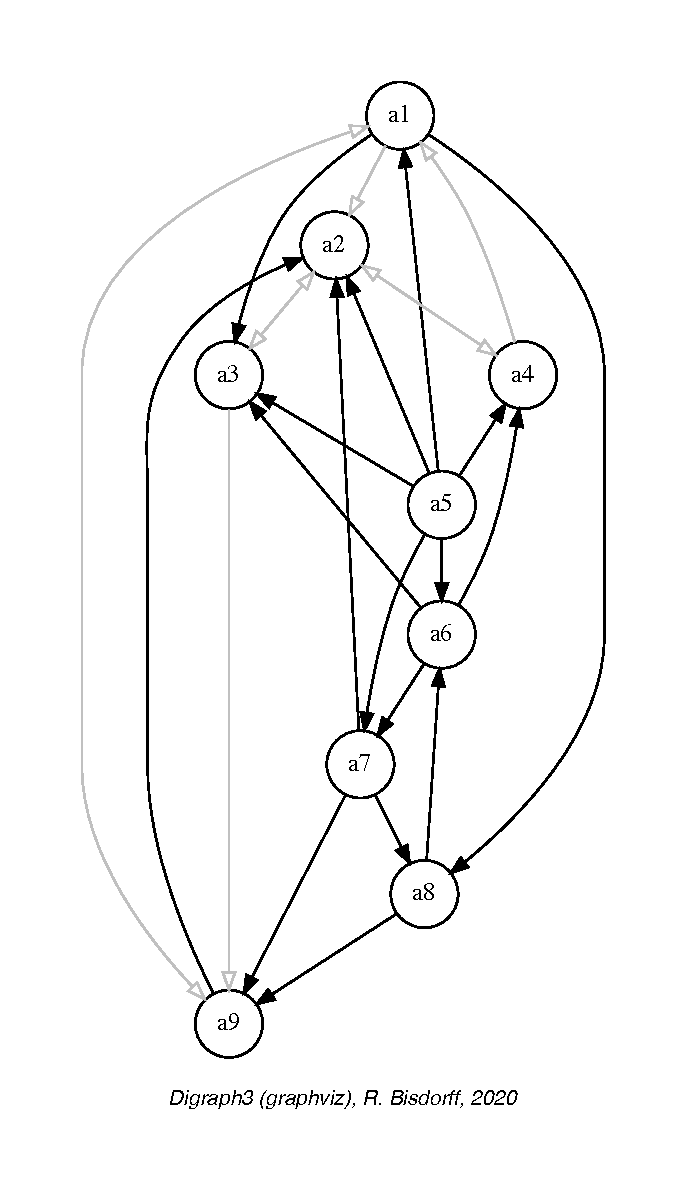
\includegraphics[width=7cm]{Figures/8-1-rankingTutorial.pdf}
\caption{The strict outranking relation $\succnsim$ shown here is, for instance, \emph{not transitive}: alternative \texttt{a8} outranks alternative \texttt{a6} and alternative \texttt{a6} outranks \texttt{a4}, however, \texttt{a8} does not outrank \texttt{a4}. Furthermore, alternatives \texttt{a6}, \texttt{a7} and \texttt{a8} show a cyclic outranking relation}
\label{fig:8.1}       % Give a unique label
\end{figure}

The \texttt{computeTransitivityDegree()} method\index{computeTransitivityDegree@\texttt{computeTransitivityDegree()}} computes the \emph{transitivity degree} of the outranking digraph shown in Figure~\vref{fig:8.1}, i.e. the ratio of the difference between the number of outranking arcs and the number of transitive arcs over the difference of the number of arcs of the transitive closure minus the transitive arcs of the digraph \texttt{gcd}.
\begin{lstlisting}
>>> gcd.computeTransitivityDegree(Comments=True)
 Transitivity degree of graph <codual_rel_randomCBperftab>
  triples x>y>z: 78, closed: 38, open: 40
  closed/triples = 0.487
\end{lstlisting}    

With only $49\%$ of the required transitive arcs, the strict outranking relation here is hence very far from being transitive; a serious problem when a linear ordering of the decision alternatives is looked for.

Let us furthermore check whether there are any cyclic outranking situations.
\begin{lstlisting}
>>> gcd.computeChordlessCircuits()
>>> gcd.showChordlessCircuits()
  1 circuit(s).
  *---- Chordless circuits ----*    
  1: ['a6', 'a7', 'a8'] , credibility : 0.033
\end{lstlisting}

There is one chordless circuit detected in the given strict outranking digraph \texttt{gcd}, namely alternative \texttt{a6} outranks alternative \texttt{a7}, the latter outranks \texttt{a8}, and \texttt{a8} outranks again alternative \texttt{a6} (see Fig.~\vref{fig:8.1}). Any potential linear ordering of these three alternatives will, in fact, always contradict somehow the given outranking relation.

Now, several heuristic ranking rules have been proposed for constructing a linear ordering which is closest in some specific sense to a given outranking relation. The \Digraph resources provide some of the most common of these ranking rules, like the \Copeland, \Kemeny, \Slater, \Kohler, and the \RankedPairs ranking rules.

\section{The \Copeland ranking}
\label{sec:8.2}

\begin{definition}[\Copeland ranking rule]\label{def:8.1}

\noindent The \Copeland ranking rule computes for each alternative a score resulting from the sum of the differences between the crisp \emph{strict outranking} characteristics $r(x\, \succnsim \,y)_{>0}$ and the crisp \emph{strict outranked} characteristics $r(y\, \succnsim \, x)_{>0}$  for all pairs of alternatives where $y$ is different from $x$. The alternatives are ranked in decreasing order of these \Copeland scores; ties, the case given, being resolved with a lexicographical rule applied to the identifiers of the alternatives \citep{COP-1951}.
\end{definition}

The \Copeland rule works well for any strict outranking relation which models a linear partial order on the \emph{median cut} strict outranking digraph \texttt{ccd} \citep{DIA-2010}. 
\begin{lstlisting}[caption={Computing a \Copeland Ranking},label=list:8.3]
>>> from linearOrders import CopelandRanking
>>> cop = CopelandRanking(gcd,Comments=True)
 Copeland decreasing scores
     a5 : +12
     a1 :  +2
     a6 :  +2
     a7 :  +2
     a8 :   0
     a4 :  -3
     a9 :  -3
     a3 :  -5
     a2 :  -7
  Copeland Ranking:
  ['a5','a1','a6','a7','a8','a4','a9','a3','a2']
\end{lstlisting}

Alternative \texttt{a5} obtains here the best \Copeland score ($+12$), followed by alternatives \texttt{a1}, \texttt{a6} and \texttt{a7} with same score ($+2$); following the lexicographic rule, \texttt{a1} is hence ranked before \texttt{a6} and \texttt{a6} before \texttt{a7}. Same situation is observed for \texttt{a4} and \texttt{a9} with a score of $-3$ (see List.~\vref{list:8.3} Lines 4-12). The \Copeland ranking rule is in fact \emph{invariant} under the \emph{codual} transform (see Sec.~\ref{sec:2.6}) and renders a same linear order indifferently from digraphs \texttt{g} or \texttt{gcd} .

In Listing~\vref{list:8.4}, the \texttt{computeRankingCorrelation()} method\index{computeRankingCorrelation@\texttt{computeRankingCorrelation()}} with the showCorrelation() method, indicate the ordinal correlation of the \Copeland ranking result, shown in Listing~\vref{list:8.3} Line 14, with the given pairwise outrankin digraph (see Chap.~\ref{sec:16} and \citet{BIS-2012a}).
\begin{lstlisting}[caption={Checking the quality of the \Copeland ranking},label=list:8.4]
>>> corr = g.computeRankingCorrelation(cop.copelandRanking)
>>> g.showCorrelation(corr)
 Correlation indexes:
   Crisp ordinal correlation : +0.463
   Valued equivalalence      : +0.107
   Epistemic determination   :  0.230
\end{lstlisting}

With an epistemic determination level of $0.230$ (Line 6), the crisp ordinal correlation --\Kendall $\tau$-- index of $+463$ is in fact supported by $61.5\% (100.0 x (1.0 + 0.23)/2)$ of the criteria significance weights. Furthermore, the bipolar-valued \emph{relational equivalence} characteristics between the strict outranking relation and the \Copeland ranking equals $+0.107$, i.e. a \emph{majority} of $55.35\%$ of the criteria significance supports the relational equivalence between the given strict outranking relation and the \Copeland ranking (see Chap.~\ref{sec:16}).

The \Copeland scores, shown in Listing~\vref{list:8.3} deliver actually only a \emph{weak ranking}, i.e. a ranking with ties. This weak ranking may be constructed with the \texttt{WeakCopelandOrder} class \index{WeakCopelandOrder@\texttt{WeakCopelandOrder} class} from the \texttt{transitiveDigraphs} module.\index{transitiveDigraphs@\texttt{transitiveDigraphs} module}
\begin{lstlisting}[caption={Computing a weak \Copeland ranking},label=list:8.5]
>>> from transitiveDigraphs import WeakCopelandOrder
>>> wcop = WeakCopelandOrder(g)
>>> wcop.showRankingByChoosing()
 Ranking by Choosing and Rejecting
   1st ranked ['a5']
     2nd ranked ['a1', 'a6', 'a7']
       3rd ranked ['a8']
       3rd last ranked ['a4', 'a9']
     2nd last ranked ['a3']
   1st last ranked ['a2']
\end{lstlisting}

We recover in Listing~\vref{list:8.5}, the preorder delivered by the \Copeland scores (see Listing~\vref{list:8.3}). We may draw its corresponding skeleton\footnote{The skeleton of a transitive relation drops the transitivity induced arcs.}.
\begin{lstlisting}
>>> wcop.exportGraphViz(fileName='weakCopelandRanking')
 *---- exporting a dot file for GraphViz tools ---------*
  Exporting to weakCopelandRanking.dot
  dot -Grankdir=TB -Tpng weakCopelandRanking.dot\
                   -o weakCopelandRanking.png
\end{lstlisting}
\begin{figure}[h]
\sidecaption[t]
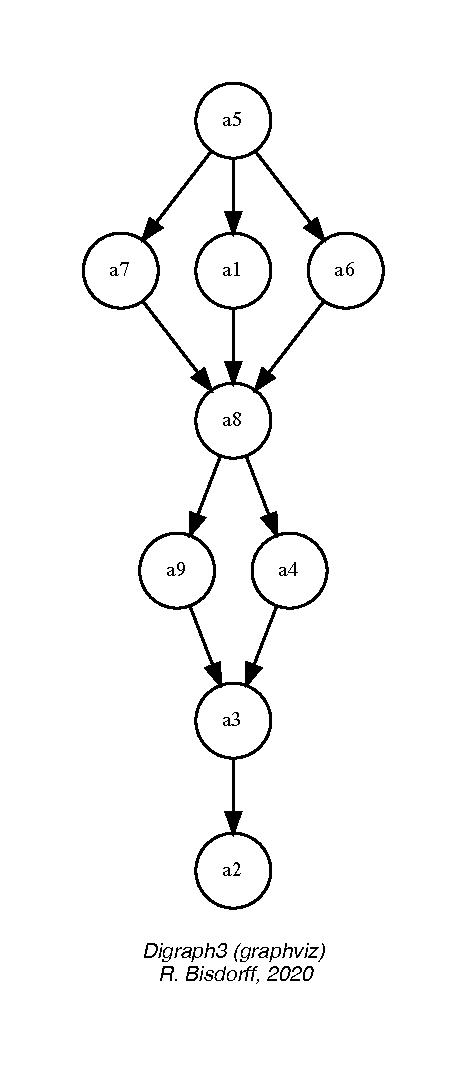
\includegraphics[width=5cm]{Figures/8-2-weakCopelandRanking.pdf}
\caption{Drawing of the weak \Copeland ranking. The graph show the skeleton of the preorder produced by the corresponding ties of the \Copeland scores}
\label{fig:8.2}       % Give a unique label
\end{figure}

Let us now consider a similar ranking rule, but working directly on the criteria \emph{significance majority margins}, i.e. the \emph{bipolar-valued} outranking relations.

\section{The \NetFlows ranking}
\label{sec:8.3}

\begin{definition}[\NetFlows ranking rule]\label{def:8.3}

\noindent The bipolar-valued version of the \Copeland ranking rule, we call \NetFlows \footnote{This ranking rule is also known under the name \Promethee ranking rule \citep*{BRA-1985}.}, computes for each alternative $x$ a \emph{net-flow} score,  i.e. the sum of the differences between the \emph{strict outranking} characteristics $r(x\, \succnsim \,y)$ and the \emph{strict outranked} characteristics $r(y\, \succnsim \,x)$ for all non-reflexive pairs of alternatives.
\end{definition}

The \texttt{NetFlowsRanking} class\index{NetFlowsRanking@\texttt{NetFlowsRanking} class} from the \texttt{linearOrders} module computes the \NetFlows ranking from a given outranking digraph.
\begin{lstlisting}[caption={Computing a \NetFlows ranking},label=list:8.6]
>>> from linearOrders import NetFlowsRanking
>>> nf = NetFlowsRanking(gcd,Comments=True)
  Net flow scores :
    a5 : +3.600
    a7 : +2.800
    a6 : +1.300
    a3 : +0.033
    a1 : -0.400
    a8 : -0.567
    a4 : -1.283
    a9 : -2.600
    a2 : -2.883
  NetFlows Ranking:
   ['a5','a7','a6','a3','a1','a8','a4','a9','a2']
>>> cop.copelandRanking # comparing both
   ['a5','a1','a6','a7','a8','a4','a9','a3','a2']
\end{lstlisting}

In our example here, the net-flows scores actually deliver a linear ranking \emph{without ties} which is rather different from the one delivered by the \Copeland rule (see List.~\vref{list:8.6} Line 16). It may happen, however, that we obtain, as with the \Copeland scores above, only a ranking with ties, which may then be resolved similarly by following a lexicographic rule applied to the identifiers of the decision alternatives. In such cases, it is possible to construct again a \emph{weak ranking} with the corresponding \texttt{WeakNetFlowsOrder} class\index{WeakNetFlowsOrder@\texttt{WeakNetFlowsOrder} class} from the \texttt{transitiveDigraphs} module.\index{transitiveDigraphs@\texttt{transitiveDigraphs} module}

It is worthwhile noticing again, that similar to the \Copeland ranking rule seen before, the \NetFlows ranking rule is also \emph{invariant} under the codual transform (see Sec.~\ref{sec:2.6}) and delivers again the same ranking result indifferently from digraphs \texttt{g} or \texttt{gcd} (see List.~\vref{list:8.6} Line 14). 

The \NetFlows ranking result appears to be slightly better correlated ($+0.638$) with the given strict outranking relation than its crisp cousin, the \Copeland ranking (see Lines 4-6 in List.~\vref{list:8.7}).
\begin{lstlisting}[caption={Checking the quality of the \NetFlows Ranking},label=list:8.6]   
>>> corr = gcd.computeOrdinalCorrelation(nf)
>>> gcd.showCorrelation(corr)
 Correlation indexes:
   Extended Kendall tau       : +0.638
   Epistemic determination    :  0.230
   Bipolar-valued equivalence : +0.147
\end{lstlisting}

Indeed, the ordinal correlation index of $+0.638$ leads to a bipolar-valued \emph{relational equivalence} characteristics of $+0.147$, i.e. a majority of $57.35\%$ of the criteria significance supports the relational equivalence between the given outranking digraphs $g$ or $gcd$  and the corresponding \NetFlows ranking (see Chap.~\ref{sec:16}). The weaker ranking quality of the \Copeland rule stems in this example essentially from the \emph{weakness} of the actual ranking result and our subsequent \emph{arbitrary} lexicographic resolution of the many ties given by the \Copeland scores (see Fig.~\vref{fig:8.2}).

To appreciate now the ordinal correlations of both the \Copeland and the \NetFlows rankings with the underlying strict outranking relation, it is useful to consider the '\emph{optimal}' \Kemeny and \Slater ranking rules.

\section{\Kemeny rankings}
\label{sec:8.4}

\begin{definition}[\Kemeny ranking rule]\label{def:8.3}

\noindent A \Kemeny ranking is a linear ranking without ties which is \emph{closest}, in the sense of the ordinal \Kendall distance (see Chap.~\ref{sec:16} and \citet{BIS-2012a}), to the given valued outranking digraphs \texttt{g} or \texttt{gcd} \citep{KEM-1959}. 
\end{definition}

The \texttt{KemenyRanking} class\index{KemenyRanking@\texttt{KemenyRanking} class} from the \texttt{linearOrders} module computes such a ranking which is highest possible correlated with the underlying strict outranking relation. The \Kemeny rule is also \emph{invariant} under the codual transform.

Mind that the \texttt{KemenyRanking} class constructor, in order to find a \Kemeny ranking, computes the ordinal correlation index for every permutation of the list of decision alternatives. Therefore we have limited by default the class to digraphs of order 7 and less. In Listing~\vref{list:8.8} Line 2, the \texttt{orderLimit} parameter allows to rise this limit.
\begin{lstlisting}[caption={Computing a \Kemeny ranking},label=list:8.8]   
>>> from linearOrders import KemenyRanking
>>> ke = KemenyRanking(gcd,orderLimit=9)
>>> # default orderLimit is 7
>>> ke.showRanking()
 ['a5','a6','a7','a3','a9','a4','a1','a8','a2']
>>> corr = gcd.computeOrdinalCorrelation(ke)
>>> gcd.showCorrelation(corr)
 Correlation indexes:
   Extended Kendall tau       : +0.779
   Epistemic determination    :  0.230
   Bipolar-valued equivalence : +0.179
\end{lstlisting}    

So, $+0.779$ represents the \emph{highest possible} ordinal correlation index --\emph{fitness}-- any potential linear ranking can achieve with the given pairwise outranking digraph (see List.~\vref{list:8.8} Lines 8-11).

A \Kemeny ranking may not be unique. In our example here, we obtain in fact two such \Kemeny rankings with a same \emph{maximal} \Kemeny index of $12.92$. 
\begin{lstlisting}[caption={Optimal \Kemeny rankings},label=list:8.9]
>>> ke.maximalRankings
  [['a5','a6','a7','a3','a8','a9','a4','a1','a2'],
   ['a5','a6','a7','a3','a9','a4','a1','a8','a2']]
>>> ke.maxKemenyIndex
  Decimal('12.9166667')
\end{lstlisting}

We may visualise in Figure~\vref{fig:8.3} the partial order defined by the epistemic disjunction of both optimal \Kemeny rankings by using the \texttt{RankingsFu\-sion} class\index{RankingsFusion@\texttt{RankingsFusion} class} (see Sec.~\ref{sec:2.5}).
\begin{lstlisting}[caption={Computing the epistemic disjunction of all optimal \Kemeny rankings},label=list:8.9]   
>>> from transitiveDigraphs import RankingsFusion
>>> wke = RankingsFusion(ke,ke.maximalRankings)
>>> wke.exportGraphViz(fileName='tutorialKemeny')
 *---- exporting a dot file for GraphViz tools ---------*
  Exporting to tutorialKemeny.dot
  dot -Grankdir=TB -Tpng tutorialKemeny.dot -o tutorialKemeny.png
\end{lstlisting}
\begin{figure}[ht]
\sidecaption[t]
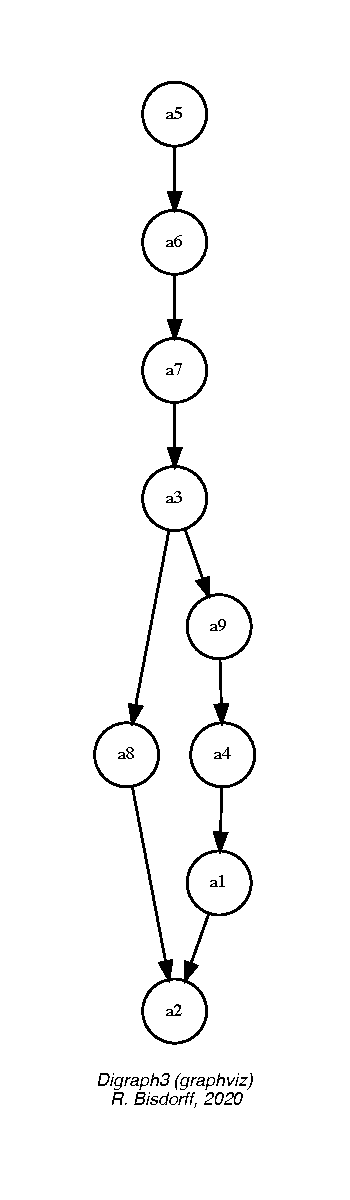
\includegraphics[width=5cm]{Figures/8-3-tutorialKemeny.pdf}
\caption{Epistemic disjunction of optimal \Kemeny rankings. It is interesting to notice that both \Kemeny rankings only differ in their respective positioning of alternative \texttt{a8}; either before or after alternatives \texttt{a9}, \texttt{a4} and \texttt{a1}}
\label{fig:8.3}       % Give a unique label
\end{figure}

To retain now a specific representative among all the potential rankings with maximal \Kemeny index, we will choose, with the help of the \texttt{showRankingCon\-sensusQuality()} method\index{showRankingConsensusQuality@Showrankingconsensusquality()}, the one proposing the best criteria consensus.
\begin{lstlisting}[caption={Computing the consensus quality of a ranking},label=list:8.10]   
>>> g.showRankingConsensusQuality(ke.maximalRankings[0])
 Consensus quality of ranking:
  ['a5','a6','a7','a3','a8','a9','a4','a1','a2']
  criterion (weight): correlation
  -------------------------------
      b09 (0.050)  : +0.361
      b04 (0.050)  : +0.333
      b08 (0.050)  : +0.292
      b01 (0.050)  : +0.264
      c01 (0.167)  : +0.250
      b03 (0.050)  : +0.222
      b07 (0.050)  : +0.194
      b05 (0.050)  : +0.167
      c02 (0.167)  : +0.000
      b10 (0.050)  : +0.000
      b02 (0.050)  : -0.042
      b06 (0.050)  : -0.097
      c03 (0.167)  : -0.167
  Summary:
    Weighted mean marginal correlation (a): +0.099
    Standard deviation (b)                : +0.177
    Ranking fairness (a)-(b)              : -0.079
>>> g.showRankingConsensusQuality(ke.maximalRankings[1])
 Consensus quality of ranking:
  ['a5','a6','a7','a3','a9','a4','a1','a8','a2']
  criterion (weight): correlation
  -------------------------------
      b09 (0.050)   : +0.306
      b08 (0.050)   : +0.236
      c01 (0.167)   : +0.194
      b07 (0.050)   : +0.194
      c02 (0.167)   : +0.167
      b04 (0.050)   : +0.167
      b03 (0.050)   : +0.167
      b01 (0.050)   : +0.153
      b05 (0.050)   : +0.056
      b02 (0.050)   : +0.014
      b06 (0.050)   : -0.042
      c03 (0.167)   : -0.111
      b10 (0.050)   : -0.111
  Summary:
    Weighted mean marginal correlation (a): +0.099
    Standard deviation (b)                : +0.132
    Ranking fairness (a)-(b)              : -0.033
\end{lstlisting}

Both \Kemeny rankings show the same \emph{weighted mean marginal correlation}: $+0.099$ with all thirteen performance criteria. However, the second ranking shows a slightly lower \emph{standard deviation}: $+0.132$ versus $+0.177$, resulting in a slightly \emph{fairer} ranking result: $-0.033$ versus $-0.079$ (see Listing~\vref{list:8.10} Lines 20-23, 42-44) .

When several rankings with maximal \Kemeny index are given, the \texttt{Kemeny\-Ranking} class constructor instantiates the ranking with \emph{highest} mean marginal correlation and, in case of ties, with \emph{lowest} weighted standard deviation. Here we obtain ranking: [\texttt{a5}, \texttt{a6}, \texttt{a7}, \texttt{a3}, \texttt{a9}, \texttt{a4}, \texttt{a1}, \texttt{a8}, \texttt{a2}] (see Line 4 in Listing~\vref{list:8.8} above).

\section{\Slater rankings}
\label{sec:8.5}

The \Slater ranking rule is identical to the \Kemeny rule, but it is working, instead, on the \Condorcet --\emph{median cut polarised}-- digraph \texttt{ccd} \citep{SLA-1961}. The \Slater rule is again \emph{invariant} under the codual transform and delivers hence indifferently on \texttt{g} or \texttt{gcd} the following results:
\begin{lstlisting}[caption={Computing a \Slater ranking},label=list:8.11]   
>>> from linearOrders import SlaterRanking
>>> sl = SlaterRanking(gcd,orderLimit=9)
>>> sl.slaterRanking
  ['a5','a6','a4','a1','a3','a7','a8','a9','a2']
>>> corr = gcd.computeRankingCorrelation(sl.slaterRanking)
>>> sl.showCorrelation(corr)
  Correlation indexes:
   Extended Kendall tau       : +0.676
   Epistemic determination    :  0.230
   Bipolar-valued equivalence : +0.156
>>> len(sl.maximalRankings)
  7
\end{lstlisting}

We notice in Listing~\vref{list:8.11} that the \Slater ranking shown in Line 4 represents a rather good fit ($+0.676$), slightly better apparently than the \NetFlows ranking result ($+0.638$). However, there are in fact 7 such optimal \Slater rankings (see Line 12). The corresponding epistemic disjunction gives the partial ordering shown in Fig~\vref{fig:8.4}:
\begin{lstlisting}[caption={Computing the epistemic disjunction of optimal \Slater rankings},label=list:8.12]   
>>> slw = RankingsFusion(sl,sl.maximalRankings)
>>> slw.exportGraphViz(fileName='tutorialSlater')
 *---- exporting a dot file for GraphViz tools ----*
  Exporting to tutorialSlater.dot
  dot -Grankdir=TB -Tpng tutorialSlater.dot\
                   -o tutorialSlater.png
\end{lstlisting}
\begin{figure}[ht]
\sidecaption[t]
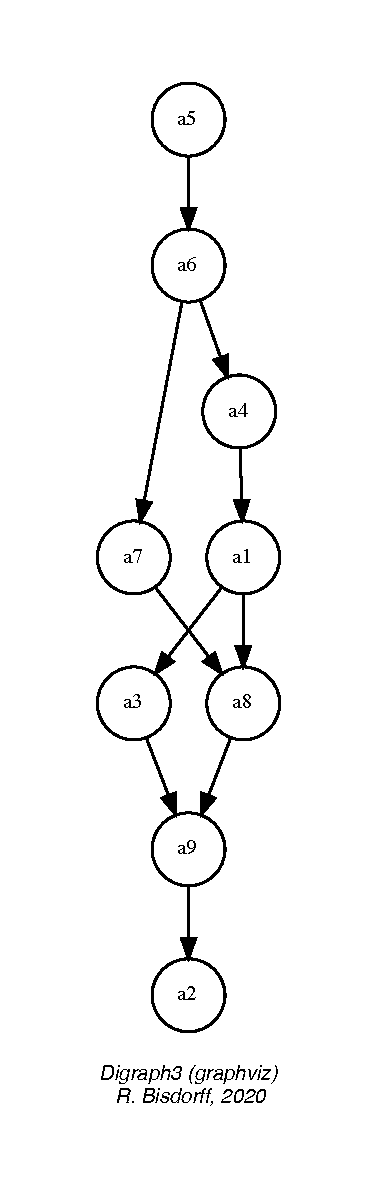
\includegraphics[width=5cm]{Figures/8-4-tutorialSlater.pdf}
\caption{Epistemic disjunction of optimal \Slater rankings. What precise \Slater ranking result should we hence adopt?}
\label{fig:8.4}       % Give a unique label
\end{figure}
       
The \Kemeny and \Slater ranking rules are furthermore computationally \emph{difficult} problems and effective ranking results are only computable for tiny outranking digraphs ($< 20$ objects). 

More efficient ranking heuristics, like the \Copeland and the \NetFlows rules, are therefore needed in practice. Let us finally, after these \emph{ranking-by-scoring} strategies, also present two popular \emph{ranking-by-choosing} strategies.

\section{The \Kohler ranking-by-choosing rule}
\label{sec:8.6}

\begin{definition}[The \Kohler \emph{ranking-by-choosing} rule]\label{def:8.4}
  
\noindent At step $i$ ($i$ goes from 1 to $n$) do the following:
\begin{enumerate}[leftmargin=0.5cm,rightmargin=0.5cm,topsep=1pt]
\item Compute for each row of the bipolar-valued \emph{strict} outranking relation table (see Listing~\vref{list:8.1}) the smallest value;
\item Select the row where this minimum is maximal. Ties are resolved in lexicographic order;
\item Put the selected decision alternative at rank $i$;
\item Delete the corresponding row and column from the relation table and restart until the table is empty.
\end{enumerate}
\end{definition}
\begin{lstlisting}[caption={Computing a \Kohler ranking},label=list:8.13]   
>>> from linearOrders import KohlerRanking
>>> kocd = KohlerRanking(gcd)
>>> kocd.showRanking()
  ['a5','a7','a6','a3','a9','a8','a4','a1','a2']
>>> corr = gcd.computeOrdinalCorrelation(kocd)
>>> gcd.showCorrelation(corr)
  Correlation indexes:
    Extended Kendall tau       : +0.747
    Epistemic determination    :  0.230
    Bipolar-valued equivalence : +0.172
\end{lstlisting}

With this \emph{min-max} lexicographic ranking-by-choosing strategy, we find a correlation result ($+0.747$) that is until now clearly the nearest to an optimal \Kemeny ranking (see Listing~\vref{list:8.8}). Only two adjacent pairs: (\texttt{a6}, \texttt{a7}) and (\texttt{a8}, \texttt{a9}) are actually inverted here. Notice that the \Kohler ranking rule, contrary to the previously mentioned rules, is \textbf{not} invariant under the codual transform and requires to work on the \texttt{strict} outranking digraph \texttt{gcd} for a better correlation result.
\begin{lstlisting}
>>> ko = KohlerRanking(g)  
>>> corr = g.computeOrdinalCorrelation(ko)
>>> g.showCorrelation(corr)
  Correlation indexes:
   Crisp ordinal correlation  : +0.483
   Epistemic determination    :  0.230
   Bipolar-valued equivalence : +0.111
\end{lstlisting}

But the \Kohler rule has a \emph{dual} version, the prudent \emph{Arrow-Raynaud} ordering-by-choosing rule, where a corresponding \emph{max-min} strategy, when used on the \emph{non-strict} outranking digraph $g$, for ordering from \emph{last} to \emph{first} produces a similar ranking result \citep{ARR-1986}.

Noticing that the \NetFlows score of an alternative $x$ represents in fact a bipolar-valued characteristic of the assertion ``\emph{alternative x is ranked first}'', we may enhance the \Kohler rule by replacing the simple \emph{min-max} strategy with an \emph{iterated} maximal \NetFlows score selection.

\begin{definition}[The iterated \NetFlows ranking-by-choosing rule]
  
\noindent At step $i$ ($i$ goes from 1 to $n$) do the following:
\begin{enumerate}[leftmargin=0.5cm,rightmargin=0.5cm]
\item Compute for each row of the bipolar-valued outranking relation table (see Listing~\vref{list:8.1}) the corresponding \NetFlows score;
\item Select the row where this score is \emph{maximal}, ties being resolved by lexicographic order;
\item Put the corresponding decision alternative at rank $i$;
\item Delete the corresponding row and column from the relation table and restart until the table is empty.
\end{enumerate}
\end{definition}

The \texttt{IteratedNetFlowsRanking}\index{IteratedNetFlowsRanking@\texttt{IteratedNetFlowsRanking} class} class from the \texttt{linearOrders} module computes this ranking result. 
\begin{lstlisting}[caption={Ranking-by-choosing with iterated maximal \NetFlows scores},label=list:8.14]   
>>> from linearOrders import IteratedNetFlowsRanking  
>>> inf = IteratedNetFlowsRanking(g)
>>> inf
 *------- Digraph instance description ------*
   Instance class      : IteratedNetFlowsRanking
   Instance name       : rel_randomCBperftab_ranked
   Digraph Order       : 9
   Digraph Size        : 36
   Valuation domain    : [-1.00;1.00]
   Determinateness (%) : 100.00
   Attributes     : ['valuedRanks', 'valuedOrdering',
                     'iteratedNetFlowsRanking',
                     'iteratedNetFlowsOrdering',
                     'name', 'actions', 'order',
                     'valuationdomain', 'relation',
                     'gamma', 'notGamma']
>>> inf.iteratedNetFlowsRanking
  ['a5','a7','a6','a3','a4','a1','a8','a9','a2']
>>> corr = g.computeRankingCorrelation(\
...             inf.iteratedNetFlowsRanking)
>>> g.showCorrelation(corr)
  Correlation indexes:
    Crisp ordinal correlation  : +0.743
    Epistemic determination    :  0.230
    Bipolar-valued equivalence : +0.171
\end{lstlisting}

Like the \Kohler rule, the iterated \NetFlows rule has also a dual \emph{ordering-by-choosing} version, where instead of choosing at each step $i$ the row with maximal \NetFlows score, we choose the row with the \emph{minimal} \NetFlows score. Both the ranking and ordering result are computed by the \texttt{IteratedNetFlowsRanking} class (see Lines 12 and 13 in Listing~\vref{list:8.14}).
\begin{lstlisting}
>>> inf.iteratedNetFlowsOrdering
  ['a2','a9','a1','a4','a3','a8','a7','a6','a5']
>>> corr = g.computeOrderCorrelation(\
...                inf.iteratedNetFlowsOrdering)
>>> g.showCorrelation(corr)
  Correlation indexes:
    Crisp ordinal correlation  : +0.751
    Epistemic determination    : 0.230
    Bipolar-valued equivalence : +0.173
\end{lstlisting}

The iterated \NetFlows ranking and its dual, the iterated \NetFlows ordering, do not usually deliver both the same result. With our example outranking digraph $g$ for instance, it is the \emph{ordering-by-choosing} result who obtains a slightly better correlation with the given outranking digraph ($+0.751$), a result that is also slightly better than the original \Kohler ranking result ($+0.747$, see Listing~\vref{list:8.13} Line 8).

With different \emph{ranking-by-choosing} and \emph{ordering-by-choosing} results, it may be useful to \emph{fuse} now, similar to what we have done before with \Kemeny 's and \Slater 's optimal rankings, both, the iterated \NetFlows ranking and ordering into a partial ranking. But we are hence back to the practical problem of what linear ranking should we eventually retain? 

Let us finally mention another interesting \emph{ranking-by-choosing} approach.

\section{The \RankedPairs ranking rule}
\label{sec:8.7}

\emph{N. Tideman}'s \index{Tideman@\emph{Tideman}} ranking-by-choosing heuristic, the \RankedPairs rule, working best this time on the non strict outranking digraph $g$, is based on a \emph{prudent incremental} construction of linear orders that avoids on the fly any cycling outranking situations \citep{TID-1987}.

\begin{definition}[The \RankedPairs ranking rule]\label{def:8.5}
\begin{enumerate}[leftmargin=0.5cm,rightmargin=0.5cm]
 \item Rank the ordered pairs $(x,y)$ of alternatives in decreasing order of $r(x\, \succsim \,y) \,+\, r(y\, \not\succsim \,x)$;
 \item Consider the pairs in that order (ties are resolved by a lexicographic rule):
   \begin{itemize}[nosep]
     \item if the next pair does not create a \emph{circuit} with the pairs already blocked, block this pair;
     \item if the next pair creates a \emph{circuit} with the already blocked pairs, skip it.
    \end{itemize}
\end{enumerate}
\end{definition}  

With our didactic outranking digraph $g$, we get the following result.\index{RankedPairsRanking@\texttt{RankedPairsRanking} class}
\begin{lstlisting}[caption={Computing a \RankedPairs ranking},label=list:8.15]   
>>> from linearOrders import RankedPairsRanking
>>> rp = RankedPairsRanking(g)
>>> rp.showRanking()
  ['a5','a6','a7','a3','a8','a9','a4','a1','a2']
\end{lstlisting}

The \RankedPairs rule renders in our example here luckily one of the two optimal \Kemeny ranking, as we may verify below.
 \begin{lstlisting}
>>> ke.maximalRankings
  [['a5','a6','a7','a3','a8','a9','a4','a1','a2'],
   ['a5','a6','a7','a3','a9','a4','a1','a8','a2']]
>>> corr = g.computeOrdinalCorrelation(rp)
>>> g.showCorrelation(corr)
  Correlation indexes:
    Extended Kendall tau       : +0.779
    Epistemic determination    :  0.230
    Bipolar-valued equivalence : +0.179
\end{lstlisting}

Similar to \Kohler 's rule, the \RankedPairs rule has also a prudent dual version, the \emph{Dias-Lamboray} \emph{ordering-by-choosing} rule, which produces, when working this time on the codual strict outranking digraph gcd, a similar ranking result (see \citet*{LAM-2009,DIA-2010}).

Besides of not providing a unique linear ranking, the \emph{ranking-by-choosing} rules, as well as their duals, the \emph{ordering-by-choosing} rules, are unfortunately not scalable to outranking digraphs of larger orders ($> 100$). For such bigger outranking digraphs, with several hundred or thousands of alternatives, only the \Copeland and the \NetFlows \emph{ranking-by-scoring} rules, with a polynomial complexity of $\mathcal{O}(n^2)$, where $n$ is the order of the outranking digraph, remain in fact tractable. Furthermore, as computing the \Copeland and \NetFlows scores may be done separately per alternative, the latter ranking rules can right away be processed in parallel when multiprocessing resources are available.

\vspace{1cm}
The physical necessity to write down a list of items in a linear sequence renders the ranking decision problem very important in practice. Concerning however the representation of preferences, a relative rating of such items into performance quantiles classes may be more expressive and faithful. This is the subject of the following Chapter~\ref{sec:10}.


%%%%%%% The chapter bibliography
%\normallatexbib
\clearpage
%\phantomsection
%\addcontentsline{toc}{section}{Chapter Bibliography}
\bibliographystyle{spbasic}
%\typeout{}
\bibliography{03-backMatters/reference}
%\chapter{Ranking with multiple incommensurable criteria}
\label{sec:8}

\abstract*{ The \Digraph python resources provide several algorithms for solving the multiple incommensurable criteria ranking problem via bipolar-valued outranking digraphs. The \Copeland, \NetFlows, \Kemeny, \Slater, \Kohler, and the \RankedPairs ranking rules are introduced and illustrated with a random outranking digraph instance.}

\begin{quotation}''... \emph{whether we are deciding between buying different commodity baskets, or making choices about what to do on a holiday, or deciding for whom to vote for in an election, we are inescapably involved in evaluating alternatives with non–commensurable aspects}.''

  --\emph{Amartya Sen}, Idea of Justice, \citep{SEN-2009}\index{Sen@\emph{A. Sen}}
\end{quotation}
\vspace{1cm}

\abstract{The \Digraph python resources provide several algorithms for solving the multiple incommensurable criteria ranking problem via bipolar-valued outranking digraphs. The \Copeland, \NetFlows, \Kemeny, \Slater, \Kohler, and the \RankedPairs ranking rules are introduced and illustrated with a random outranking digraph.}

\section{The ranking problem}
\label{sec:8.1}

We need to rank without ties a set $X$ of items (usually decision alternatives) that are evaluated on multiple incommensurable performance criteria; yet, for which we may know their pairwise bipolar-valued \emph{strict outranking} characteristics, i.e. $r(x\, \succnsim \, y)$ for all $x, y \in X$ (see Sec.~\ref{sec:3.5} and \citep{BIS-2013}).

Let us consider in Listing~\vref{list:8.1} a didactic outranking digraph \texttt{g} generated from a random \emph{Cost-Benefit} performance tableau (see Sec.~\ref{sec:6.3}) concerning 9 decision alternatives evaluated on 13 performance criteria. We can compute the corresponding \emph{strict outranking digraph} with a codual transform (see Sec. ~\ref{sec:2.6}).
\begin{lstlisting}[caption={Random bipolar-valued strict outranking relation characteristics},label=list:8.1]
>>> from randomPerfTabs import RandomCBPerformanceTableau   
>>> t = RandomCBPerformanceTableau(numberOfActions=9,\
...         numberOfCriteria=13,seed=200)
>>> from outrankingDigraphs import BipolarOutrankingDigraph
>>> g = BipolarOutrankingDigraph(t)
>>> gcd = ~(-g) # codual digraph
>>> gcd.showRelationTable(ReflexiveTerms=False)
 * ---- Relation Table -----
  r(>) |  'a1'  'a2'  'a3'  'a4'  'a5'  'a6'  'a7'  'a8'  'a9'   
  -----|------------------------------------------------------
  'a1' |    -   0.00 +0.10 -1.00 -0.13 -0.57 -0.23 +0.10 +0.00  
  'a2' | -1.00   -    0.00 +0.00 -0.37 -0.42 -0.28 -0.32 -0.12  
  'a3' | -0.10  0.00   -   -0.17 -0.35 -0.30 -0.17 -0.17 +0.00  
  'a4' |  0.00  0.00 -0.42   -   -0.40 -0.20 -0.60 -0.27 -0.30  
  'a5' | +0.13 +0.22 +0.10 +0.40   -   +0.03 +0.40 -0.03 -0.07  
  'a6' | -0.07 -0.22 +0.20 +0.20 -0.37   -   +0.10 -0.03 -0.07  
  'a7' | -0.20 +0.28 -0.03 -0.07 -0.40 -0.10   -   +0.27 +1.00  
  'a8' | -0.10 -0.02 -0.23 -0.13 -0.37 +0.03 -0.27   -   +0.03  
  'a9' |  0.00 +0.12 -1.00 -0.13 -0.03 -0.03 -1.00 -0.03   -   
\end{lstlisting}
  
Some ranking rules will work on the associated \Condorcet digraph\index{Condorcet digraph}, i.e. the corresponding \emph{median cut} polarised strict outranking digraph.
 \begin{lstlisting}[caption={Median cut polarised strict outranking relation characteristics},label=list:8.2]
>>> ccd = PolarisedOutrankingDigraph(gcd,\
...                   level=g.valuationdomain['med'],\
...                   KeepValues=False,StrictCut=True)
>>> ccd.showRelationTable(ReflexiveTerms=False,\
...                       IntegerValues=True)
 *---- Relation Table -----
  r(>)_med | 'a1' 'a2' 'a3' 'a4' 'a5' 'a6' 'a7' 'a8' 'a9'   
  ---------|---------------------------------------------
     'a1'  |   -    0   +1   -1   -1   -1   -1   +1    0  
     'a2'  |  -1    -   +0    0   -1   -1   -1   -1   -1  
     'a3'  |  -1    0    -   -1   -1   -1   -1   -1    0  
     'a4'  |   0    0   -1    -   -1   -1   -1   -1   -1  
     'a5'  |  +1   +1   +1   +1    -   +1   +1   -1   -1  
     'a6'  |  -1   -1   +1   +1   -1    -   +1   -1   -1  
     'a7'  |  -1   +1   -1   -1   -1   -1    -   +1   +1  
     'a8'  |  -1   -1   -1   -1   -1   +1   -1    -   +1  
     'a9'  |   0   +1   -1   -1   -1   -1   -1   -1    -   
\end{lstlisting}

Unfortunately, such crisp median-cut \Condorcet digraphs, associated with a given strict outranking digraph, only exceptionally model a linear ordering. Usually, pairwise majority comparisons do not render a \emph{complete} or, at least, a \emph{transitive} partial order. There may even frequently appear \emph{cyclic} outranking situations (see Sec.~\ref{sec:7.4}).

To discover how \emph{difficult} this ranking problem can get, let us have a look in Figure.~\vref{fig:8.1} at the corresponding strict outranking digraph \emph{graphviz} drawing \footnote{ The \texttt{exportGraphViz()} method is depending on drawing tools from graphviz software (https://graphviz.org/).}.
\begin{lstlisting}
>>> gcd.exportGraphViz(fileName='rankingTutorial')
 *---- exporting a dot file for GraphViz tools ---------*
  Exporting to rankingTutorial.dot
  dot -Grankdir=BT -Tpng rankingTutorial.dot\
                   -o rankingTutorial.png
\end{lstlisting}
\begin{figure}[ht]
\sidecaption[t]
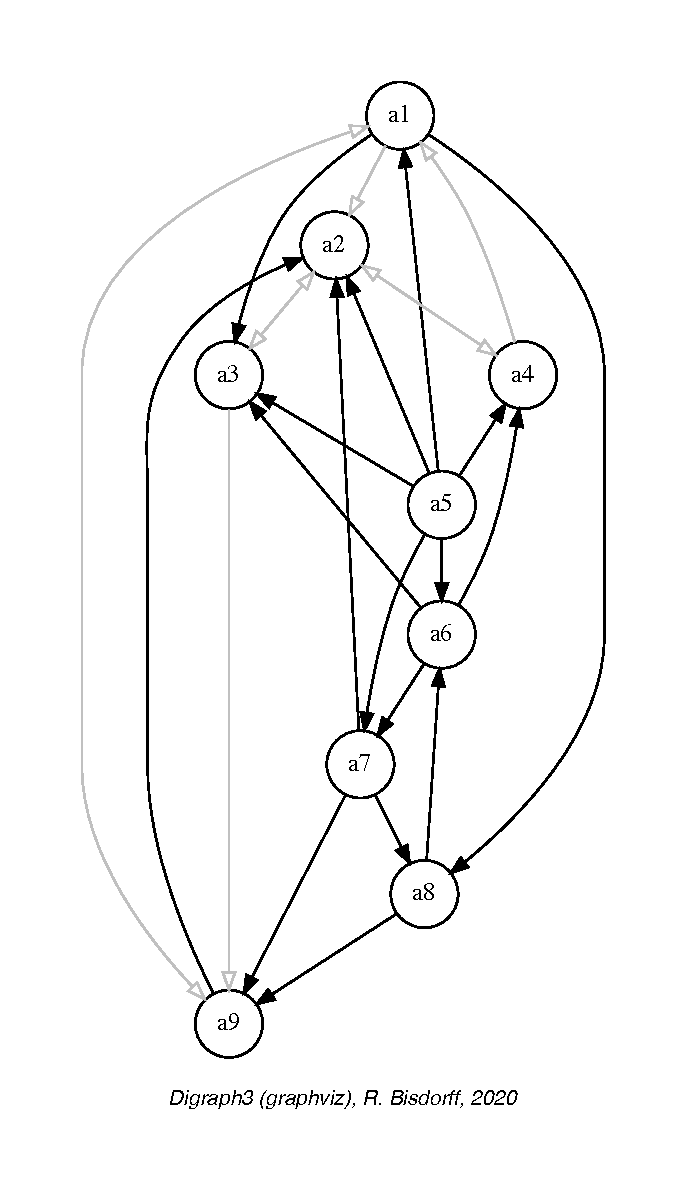
\includegraphics[width=7cm]{Figures/8-1-rankingTutorial.pdf}
\caption{The strict outranking relation $\succnsim$ shown here is, for instance, \emph{not transitive}: alternative \texttt{a8} outranks alternative \texttt{a6} and alternative \texttt{a6} outranks \texttt{a4}, however, \texttt{a8} does not outrank \texttt{a4}. Furthermore, alternatives \texttt{a6}, \texttt{a7} and \texttt{a8} show a cyclic outranking relation}
\label{fig:8.1}       % Give a unique label
\end{figure}

The \texttt{computeTransitivityDegree()} method\index{computeTransitivityDegree@\texttt{computeTransitivityDegree()}} computes the \emph{transitivity degree} of the outranking digraph shown in Figure~\vref{fig:8.1}, i.e. the ratio of the difference between the number of outranking arcs and the number of transitive arcs over the difference of the number of arcs of the transitive closure minus the transitive arcs of the digraph \texttt{gcd}.
\begin{lstlisting}
>>> gcd.computeTransitivityDegree(Comments=True)
 Transitivity degree of graph <codual_rel_randomCBperftab>
  triples x>y>z: 78, closed: 38, open: 40
  closed/triples = 0.487
\end{lstlisting}    

With only $49\%$ of the required transitive arcs, the strict outranking relation here is hence very far from being transitive; a serious problem when a linear ordering of the decision alternatives is looked for.

Let us furthermore check whether there are any cyclic outranking situations.
\begin{lstlisting}
>>> gcd.computeChordlessCircuits()
>>> gcd.showChordlessCircuits()
  1 circuit(s).
  *---- Chordless circuits ----*    
  1: ['a6', 'a7', 'a8'] , credibility : 0.033
\end{lstlisting}

There is one chordless circuit detected in the given strict outranking digraph \texttt{gcd}, namely alternative \texttt{a6} outranks alternative \texttt{a7}, the latter outranks \texttt{a8}, and \texttt{a8} outranks again alternative \texttt{a6} (see Fig.~\vref{fig:8.1}). Any potential linear ordering of these three alternatives will, in fact, always contradict somehow the given outranking relation.

Now, several heuristic ranking rules have been proposed for constructing a linear ordering which is closest in some specific sense to a given outranking relation. The \Digraph resources provide some of the most common of these ranking rules, like the \Copeland, \Kemeny, \Slater, \Kohler, and the \RankedPairs ranking rules.

\section{The \Copeland ranking}
\label{sec:8.2}

\begin{definition}[\Copeland ranking rule]\label{def:8.1}

\noindent The \Copeland ranking rule computes for each alternative a score resulting from the sum of the differences between the crisp \emph{strict outranking} characteristics $r(x\, \succnsim \,y)_{>0}$ and the crisp \emph{strict outranked} characteristics $r(y\, \succnsim \, x)_{>0}$  for all non-reflexive pairs of alternatives. The alternatives are ranked in decreasing order of these scores; ties, the case given, being resolved with a lexicographical rule applied to the identifiers of the alternatives \citep{COP-1951}.
\end{definition}

The \Copeland rule works well for any strict outranking relation which models a linear partial order on the \emph{median cut} strict outranking digraph \texttt{ccd} \citep{DIA-2010}. 
\begin{lstlisting}[caption={Computing a \Copeland Ranking},label=list:8.3]
>>> from linearOrders import CopelandRanking
>>> cop = CopelandRanking(gcd,Comments=True)
 Copeland decreasing scores
     a5 : +12
     a1 :  +2
     a6 :  +2
     a7 :  +2
     a8 :   0
     a4 :  -3
     a9 :  -3
     a3 :  -5
     a2 :  -7
  Copeland Ranking:
  ['a5','a1','a6','a7','a8','a4','a9','a3','a2']
\end{lstlisting}

Alternative \texttt{a5} obtains here the best \Copeland score ($+12$), followed by alternatives \texttt{a1}, \texttt{a6} and \texttt{a7} with same score ($+2$); following the lexicographic rule, \texttt{a1} is hence ranked before \texttt{a6} and \texttt{a6} before \texttt{a7}. Same situation is observed for \texttt{a4} and \texttt{a9} with a score of $-3$ (see List.~\vref{list:8.3} Lines 4-12). The \Copeland ranking rule is in fact \emph{invariant} under the \emph{codual} transform (see Sec.~\ref{sec:2.6}) and renders a same linear order indifferently from digraphs \texttt{g} or \texttt{gcd} .

In Listing~\vref{list:8.4}, the \texttt{computeRankingCorrelation()} method\index{computeRankingCorrelation@\texttt{computeRankingCorrelation()}}, coupled with the \texttt{showCorrelation()} method, indicate the ordinal correlation of the \Copeland ranking result, shown in Listing~\vref{list:8.3} Line 14, with the given outranking digraph \texttt{g} (see Chap.~\ref{sec:16} and \citet{BIS-2012a}).
\begin{lstlisting}[caption={Checking the ordinal quality of the \Copeland ranking},label=list:8.4]
>>> corr = g.computeRankingCorrelation(cop.copelandRanking)
>>> g.showCorrelation(corr)
 Correlation indexes:
   Crisp ordinal correlation : +0.463
   Valued equivalalence      : +0.107
   Epistemic determination   :  0.230
\end{lstlisting}

With an epistemic determination level of $0.230$ (Line 6), the crisp ordinal correlation --\Kendall $\tau$-- index of $+463$ is in fact supported by $61.5\% (100.0 x (1.0 + 0.23)/2)$ of the criteria significance weights. Furthermore, the bipolar-valued \emph{relational equivalence} characteristics between the strict outranking relation and the \Copeland ranking equals $+0.107$, i.e. a \emph{majority} of $55.35\%$ of the criteria significance supports the relational equivalence between the given strict outranking relation and the \Copeland ranking (see Chap.~\ref{sec:16}).

The \Copeland scores, shown in Listing~\vref{list:8.3} deliver actually only a \emph{weak ranking}, i.e. a ranking with ties. This weak ranking may be constructed with the \texttt{WeakCopelandOrder} class \index{WeakCopelandOrder@\texttt{WeakCopelandOrder} class} from the \texttt{transitiveDigraphs} module.\index{transitiveDigraphs@\texttt{transitiveDigraphs} module}
\begin{lstlisting}[caption={Computing a weak \Copeland ranking},label=list:8.5]
>>> from transitiveDigraphs import WeakCopelandOrder
>>> wcop = WeakCopelandOrder(g)
>>> wcop.showRankingByChoosing()
 Ranking by Choosing and Rejecting
   1st ranked ['a5']
     2nd ranked ['a1', 'a6', 'a7']
       3rd ranked ['a8']
       3rd last ranked ['a4', 'a9']
     2nd last ranked ['a3']
   1st last ranked ['a2']
\end{lstlisting}

We recover in Listing~\vref{list:8.5}, the preorder delivered by the \Copeland scores (see Listing~\vref{list:8.3}). We may draw its corresponding skeleton\footnote{The skeleton of a transitive relation drops the transitivity induced arcs.}.
\begin{lstlisting}
>>> wcop.exportGraphViz(fileName='weakCopelandRanking')
 *---- exporting a dot file for GraphViz tools ---------*
  Exporting to weakCopelandRanking.dot
  dot -Grankdir=TB -Tpng weakCopelandRanking.dot\
                   -o weakCopelandRanking.png
\end{lstlisting}
\begin{figure}[h]
\sidecaption[t]
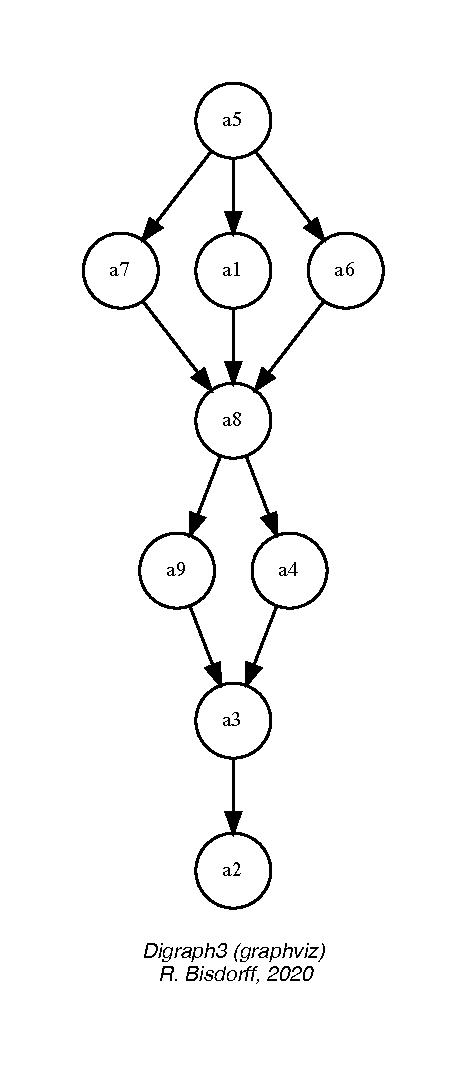
\includegraphics[width=5cm]{Figures/8-2-weakCopelandRanking.pdf}
\caption{Drawing of the weak \Copeland ranking. The graph show the skeleton of the preorder produced by the corresponding ties of the \Copeland scores}
\label{fig:8.2}       % Give a unique label
\end{figure}

Let us now consider a similar ranking rule, but working directly on the criteria \emph{significance majority margins}, i.e. the \emph{bipolar-valued} outranking relations.

\section{The \NetFlows ranking}
\label{sec:8.3}

\begin{definition}[\NetFlows ranking rule]\label{def:8.3}

\noindent The bipolar-valued version of the \Copeland ranking rule, we call \NetFlows \footnote{This ranking rule is also known under the name \Promethee ranking rule \citep*{BRA-1985}.}, computes for each alternative $x$ a \emph{net-flow} score,  i.e. the sum of the differences between the \emph{strict outranking} characteristics $r(x\, \succnsim \,y)$ and the \emph{strict outranked} characteristics $r(y\, \succnsim \,x)$ for all non-reflexive pairs of alternatives.
\end{definition}

The \texttt{NetFlowsRanking} class\index{NetFlowsRanking@\texttt{NetFlowsRanking} class} from the \texttt{linearOrders} module computes the \NetFlows ranking from a given outranking digraph.
\begin{lstlisting}[caption={Computing a \NetFlows ranking},label=list:8.6]
>>> from linearOrders import NetFlowsRanking
>>> nf = NetFlowsRanking(gcd,Comments=True)
  Net flow scores :
    a5 : +3.600
    a7 : +2.800
    a6 : +1.300
    a3 : +0.033
    a1 : -0.400
    a8 : -0.567
    a4 : -1.283
    a9 : -2.600
    a2 : -2.883
  NetFlows Ranking:
   ['a5','a7','a6','a3','a1','a8','a4','a9','a2']
>>> cop.copelandRanking # comparing both
   ['a5','a1','a6','a7','a8','a4','a9','a3','a2']
\end{lstlisting}

In our example here, the net-flows scores actually deliver a linear ranking \emph{without ties} which is rather different from the one delivered by the \Copeland rule (see List.~\vref{list:8.6} Line 16). It may happen, however, that we obtain, as with the \Copeland scores above, only a ranking with ties, which may then be resolved similarly by following a lexicographic rule applied to the identifiers of the decision alternatives. In such cases, it is possible to construct again a \emph{weak ranking} with the corresponding \texttt{WeakNetFlowsOrder} class\index{WeakNetFlowsOrder@\texttt{WeakNetFlowsOrder} class} from the \texttt{transitiveDigraphs} module.\index{transitiveDigraphs@\texttt{transitiveDigraphs} module}

It is worthwhile noticing again, that similar to the \Copeland ranking rule seen before, the \NetFlows ranking rule is also \emph{invariant} under the codual transform (see Sec.~\ref{sec:2.6}) and delivers again the same ranking result indifferently from digraphs \texttt{g} or \texttt{gcd} (see List.~\vref{list:8.6} Line 14). 

The \NetFlows ranking result appears to be slightly better correlated ($+0.638$) with the given strict outranking relation than its crisp cousin, the \Copeland ranking (see Lines 4-6 in List.~\vref{list:8.7}).
\begin{lstlisting}[caption={Checking the quality of the \NetFlows Ranking},label=list:8.7]   
>>> corr = gcd.computeOrdinalCorrelation(nf)
>>> gcd.showCorrelation(corr)
 Correlation indexes:
   Extended Kendall tau       : +0.638
   Epistemic determination    :  0.230
   Bipolar-valued equivalence : +0.147
\end{lstlisting}

Indeed, the ordinal correlation index of $+0.638$ leads to a bipolar-valued \emph{relational equivalence} characteristics of $+0.147$, i.e. a majority of $57.35\%$ of the criteria significance supports the relational equivalence between the given outranking digraphs $g$ or $gcd$  and the corresponding \NetFlows ranking (see Chap.~\ref{sec:16}). The weaker ordinal ranking quality of the \Copeland rule ($+0.463$) stems in this example here essentially from the \emph{weakness} of the actual \Copeland ranking result and our subsequent \emph{arbitrary} lexicographic resolution of the many ties given by the \Copeland scores (see Fig.~\vref{fig:8.2}).

To appreciate now the ordinal correlations of both the \Copeland and the \NetFlows rankings with the underlying strict outranking relation, it is useful to consider the '\emph{optimal}' \Kemeny and \Slater ranking rules.

\section{\Kemeny rankings}
\label{sec:8.4}

\begin{definition}[\Kemeny ranking rule]\label{def:8.3}

  \noindent A \Kemeny ranking $k$ is a linear ranking without ties of the set of $n$ decision alternatives $X$ which is \emph{closest}, in the sense of the ordinal \Kendall distance (see Chap.~\ref{sec:16} and \citet{BIS-2012b}), to the given valued outranking digraphs \texttt{g} \citep{KEM-1959}. Formally:
  \begin{equation}\label{eq:8.1}
    k \;=\; \text{argmax}_{p \in \mathcal{P}(X)} \sum_{i \neq j}\big(r(p[i] \succsim p[j]) - r(p[j] \succsim p[i]) \big),
  \end{equation}
where $\mathcal{P}(X)$ denotes the set of all permutations of $X$ and $i,j = 0,... n$.
\end{definition}

The \texttt{KemenyRanking} class\index{KemenyRanking@\texttt{KemenyRanking} class} from the \texttt{linearOrders} module computes such a ranking which is highest possible correlated with the underlying strict outranking relation. The \Kemeny rule is also \emph{invariant} under the codual transform.

Mind that the \texttt{KemenyRanking} class constructor, in order to find a \Kemeny ranking, has to compute a net-flows score for every permutation of the list of decision alternatives (see Eq.~\vref{eq:8.1}). Therefore the class is limited, by default, to digraphs of order up to 7 \citep{BIS-2021b}. In Listing~\vref{list:8.8} Line 2, the \texttt{orderLimit} parameter allows to rise this limit.
\begin{lstlisting}[caption={Computing a \Kemeny ranking},label=list:8.8]   
>>> from linearOrders import KemenyRanking
>>> ke = KemenyRanking(gcd,orderLimit=9)
>>> # default orderLimit is 7
>>> ke.showRanking()
 ['a5','a6','a7','a3','a9','a4','a1','a8','a2']
>>> corr = gcd.computeOrdinalCorrelation(ke)
>>> gcd.showCorrelation(corr)
 Correlation indexes:
   Extended Kendall tau       : +0.779
   Epistemic determination    :  0.230
   Bipolar-valued equivalence : +0.179
\end{lstlisting}    

So, $+0.779$ represents the \emph{highest possible} ordinal correlation index --\emph{fitness}-- any potential linear ranking can achieve with the given pairwise outranking digraph (see List.~\vref{list:8.8} Lines 8-11).

A \Kemeny ranking may not be unique. In our example here, we obtain in fact two such \Kemeny rankings with a same \emph{maximal} \Kemeny index of $12.92$. 
\begin{lstlisting}[caption={Optimal \Kemeny rankings},label=list:8.9]
>>> ke.maximalRankings
  [['a5','a6','a7','a3','a8','a9','a4','a1','a2'],
   ['a5','a6','a7','a3','a9','a4','a1','a8','a2']]
>>> ke.maxKemenyIndex
  Decimal('12.9166667')
\end{lstlisting}

We may visualise in Figure~\vref{fig:8.3} the partial order defined by the epistemic disjunction of both optimal \Kemeny rankings by using the \texttt{RankingsFu\-sion} class\index{RankingsFusion@\texttt{RankingsFusion} class} (see Sec.~\ref{sec:2.5}).
\begin{lstlisting}[caption={Computing the epistemic disjunction of all optimal \Kemeny rankings},label=list:8.9]   
>>> from transitiveDigraphs import RankingsFusion
>>> wke = RankingsFusion(ke,ke.maximalRankings)
>>> wke.exportGraphViz(fileName='tutorialKemeny')
 *---- exporting a dot file for GraphViz tools ---------*
  Exporting to tutorialKemeny.dot
  dot -Grankdir=TB -Tpng tutorialKemeny.dot -o tutorialKemeny.png
\end{lstlisting}
\begin{figure}[ht]
\sidecaption[t]
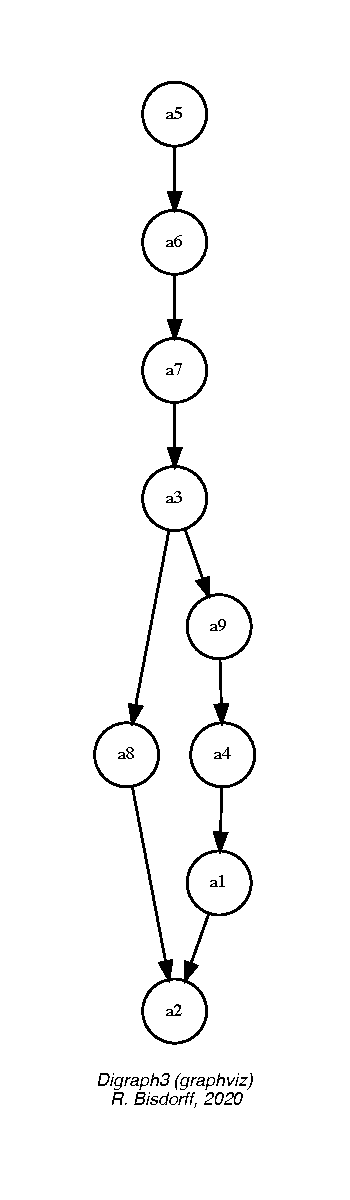
\includegraphics[width=5cm]{Figures/8-3-tutorialKemeny.pdf}
\caption{Epistemic disjunction of optimal \Kemeny rankings. It is interesting to notice that both \Kemeny rankings only differ in their respective positioning of alternative \texttt{a8}; either before or after alternatives \texttt{a9}, \texttt{a4} and \texttt{a1}}
\label{fig:8.3}       % Give a unique label
\end{figure}

To retain now a specific representative among all the potential rankings with maximal \Kemeny index, we will choose, with the help of the \texttt{showRankingCon\-sensusQuality()} method\index{showRankingConsensusQuality@Showrankingconsensusquality()}, the one proposing the best criteria consensus.
\begin{lstlisting}[caption={Computing the consensus quality of a ranking},label=list:8.10]   
>>> g.showRankingConsensusQuality(ke.maximalRankings[0])
 Consensus quality of ranking:
  ['a5','a6','a7','a3','a8','a9','a4','a1','a2']
  criterion (weight): correlation
  -------------------------------
      b09 (0.050)  : +0.361
      b04 (0.050)  : +0.333
      b08 (0.050)  : +0.292
      b01 (0.050)  : +0.264
      c01 (0.167)  : +0.250
      b03 (0.050)  : +0.222
      b07 (0.050)  : +0.194
      b05 (0.050)  : +0.167
      c02 (0.167)  : +0.000
      b10 (0.050)  : +0.000
      b02 (0.050)  : -0.042
      b06 (0.050)  : -0.097
      c03 (0.167)  : -0.167
  Summary:
    Weighted mean marginal correlation (a): +0.099
    Standard deviation (b)                : +0.177
    Ranking fairness (a)-(b)              : -0.079
>>> g.showRankingConsensusQuality(ke.maximalRankings[1])
 Consensus quality of ranking:
  ['a5','a6','a7','a3','a9','a4','a1','a8','a2']
  criterion (weight): correlation
  -------------------------------
      b09 (0.050)   : +0.306
      b08 (0.050)   : +0.236
      c01 (0.167)   : +0.194
      b07 (0.050)   : +0.194
      c02 (0.167)   : +0.167
      b04 (0.050)   : +0.167
      b03 (0.050)   : +0.167
      b01 (0.050)   : +0.153
      b05 (0.050)   : +0.056
      b02 (0.050)   : +0.014
      b06 (0.050)   : -0.042
      c03 (0.167)   : -0.111
      b10 (0.050)   : -0.111
  Summary:
    Weighted mean marginal correlation (a): +0.099
    Standard deviation (b)                : +0.132
    Ranking fairness (a)-(b)              : -0.033
\end{lstlisting}

Both \Kemeny rankings show the same \emph{weighted mean marginal correlation}: $+0.099$ with all thirteen performance criteria. However, the second ranking shows a slightly lower \emph{standard deviation}: $+0.132$ versus $+0.177$, resulting in a slightly \emph{fairer} ranking result: $-0.033$ versus $-0.079$ (see Listing~\vref{list:8.10} Lines 20-23, 42-44) .

When several rankings with maximal \Kemeny index are given, the \texttt{Kemeny\-Ranking} class constructor instantiates the ranking with \emph{highest} mean marginal correlation and, in case of ties, with \emph{lowest} weighted standard deviation. Here we obtain ranking: [\texttt{a5}, \texttt{a6}, \texttt{a7}, \texttt{a3}, \texttt{a9}, \texttt{a4}, \texttt{a1}, \texttt{a8}, \texttt{a2}] (see Line 4 in Listing~\vref{list:8.8} above).

\section{\Slater rankings}
\label{sec:8.5}

The \Slater ranking rule is identical to the \Kemeny rule, but it is working, instead, on the \Condorcet --\emph{median cut polarised}-- digraph \texttt{ccd} \citep{SLA-1961}. The \Slater rule is again \emph{invariant} under the codual transform and delivers hence indifferently on \texttt{g} or \texttt{gcd} the following results:
\begin{lstlisting}[caption={Computing a \Slater ranking},label=list:8.11]   
>>> from linearOrders import SlaterRanking
>>> sl = SlaterRanking(gcd,orderLimit=9)
>>> sl.slaterRanking
  ['a5','a6','a4','a1','a3','a7','a8','a9','a2']
>>> corr = gcd.computeRankingCorrelation(sl.slaterRanking)
>>> sl.showCorrelation(corr)
  Correlation indexes:
   Extended Kendall tau       : +0.676
   Epistemic determination    :  0.230
   Bipolar-valued equivalence : +0.156
>>> len(sl.maximalRankings)
  7
\end{lstlisting}

We notice in Listing~\vref{list:8.11} that the \Slater ranking shown in Line 4 represents a rather good fit ($+0.676$), slightly better apparently than the \NetFlows ranking result ($+0.638$). However, there are in fact 7 such optimal \Slater rankings (see Line 12). The corresponding epistemic disjunction gives the partial ordering shown in Fig~\vref{fig:8.4}:
\begin{lstlisting}[caption={Computing the epistemic disjunction of optimal \Slater rankings},label=list:8.12]   
>>> slw = RankingsFusion(sl,sl.maximalRankings)
>>> slw.exportGraphViz(fileName='tutorialSlater')
 *---- exporting a dot file for GraphViz tools ----*
  Exporting to tutorialSlater.dot
  dot -Grankdir=TB -Tpng tutorialSlater.dot\
                   -o tutorialSlater.png
\end{lstlisting}
\begin{figure}[ht]
\sidecaption[t]
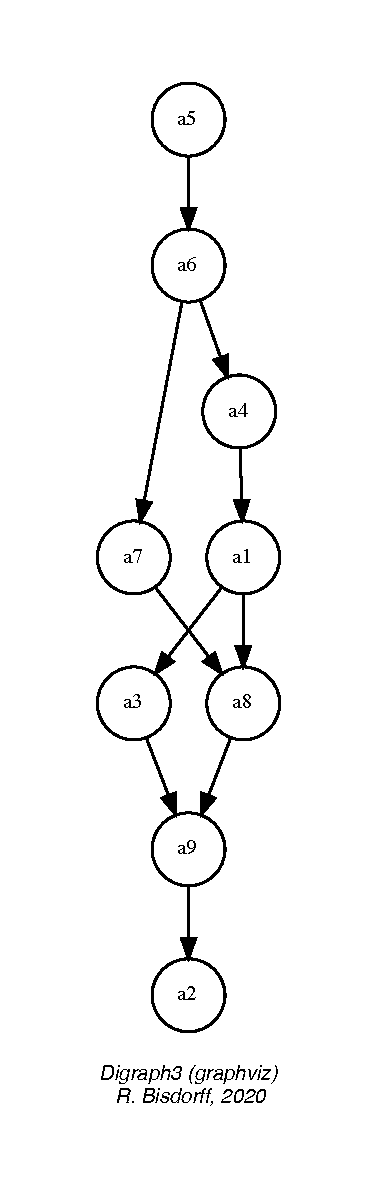
\includegraphics[width=5cm]{Figures/8-4-tutorialSlater.pdf}
\caption{Epistemic disjunction of optimal \Slater rankings. What precise \Slater ranking result should we hence adopt?}
\label{fig:8.4}       % Give a unique label
\end{figure}
       
The \Kemeny and \Slater ranking rules are furthermore computationally \emph{difficult} problems and effective ranking results are only computable for tiny outranking digraphs ($< 20$ objects) (see Eq.~\vref{eq:8.1}). 

More computationally efficient ranking heuristics, like the \Copeland and \NetFlows rules, are therefore needed in practice. Let us finally, after these \emph{ranking-by-scoring} strategies, also present two popular \emph{ranking-by-choosing} strategies.

\section{The \Kohler ranking-by-choosing rule}
\label{sec:8.6}

\begin{definition}[The \Kohler \emph{ranking-by-choosing} rule]\label{def:8.4}
  
\noindent At step $i$ ($i$ goes from 1 to $n$) do the following:
\begin{enumerate}[leftmargin=0.5cm,rightmargin=0.5cm,topsep=1pt]
\item Compute for each row of the bipolar-valued \emph{strict} outranking relation table (see Listing~\vref{list:8.1}) the smallest value;
\item Select the row where this minimum is maximal. Ties are resolved in lexicographic order;
\item Put the selected decision alternative at rank $i$;
\item Delete the corresponding row and column from the relation table and restart until the table is empty.
\end{enumerate}
\end{definition}
\begin{lstlisting}[caption={Computing a \Kohler ranking},label=list:8.13]   
>>> from linearOrders import KohlerRanking
>>> kocd = KohlerRanking(gcd)
>>> kocd.showRanking()
  ['a5','a7','a6','a3','a9','a8','a4','a1','a2']
>>> corr = gcd.computeOrdinalCorrelation(kocd)
>>> gcd.showCorrelation(corr)
  Correlation indexes:
    Extended Kendall tau       : +0.747
    Epistemic determination    :  0.230
    Bipolar-valued equivalence : +0.172
\end{lstlisting}

With this \emph{min-max} lexicographic ranking-by-choosing strategy, we find a correlation result ($+0.747$) that is until now clearly the nearest to an optimal \Kemeny ranking (see Listing~\vref{list:8.8}). Only two adjacent pairs: (\texttt{a6}, \texttt{a7}) and (\texttt{a8}, \texttt{a9}) are actually inverted here. Notice that the \Kohler ranking rule, contrary to the previously mentioned rules, is \textbf{not} invariant under the codual transform and requires to work on the \texttt{strict} outranking digraph \texttt{gcd} for a better correlation result.
\begin{lstlisting}
>>> ko = KohlerRanking(g)  
>>> corr = g.computeOrdinalCorrelation(ko)
>>> g.showCorrelation(corr)
  Correlation indexes:
   Crisp ordinal correlation  : +0.483
   Epistemic determination    :  0.230
   Bipolar-valued equivalence : +0.111
\end{lstlisting}

But the \Kohler rule has a \emph{dual} version, the prudent \emph{Arrow-Raynaud} ordering-by-choosing rule, where a corresponding \emph{max-min} strategy, when used on the \emph{non-strict} outranking digraph $g$, for ordering from \emph{last} to \emph{first} produces a similar ranking result \citep{ARR-1986}.

Noticing that the \NetFlows score of an alternative $x$ represents in fact a bipolar-valued characteristic of the assertion ``\emph{alternative x is ranked first}'', we may enhance the \Kohler rule by replacing the simple \emph{min-max} strategy with an \emph{iterated} maximal \NetFlows score selection.

\begin{definition}[The iterated \NetFlows ranking-by-choosing rule]
  
\noindent At step $i$ ($i$ goes from 1 to $n$) do the following:
\begin{enumerate}[leftmargin=0.5cm,rightmargin=0.5cm,topsep=1pt]
\item Compute for each row of the bipolar-valued outranking relation table (see Listing~\vref{list:8.1}) the corresponding \NetFlows score;
\item Select the row where this score is \emph{maximal}, ties being resolved by lexicographic order;
\item Put the corresponding decision alternative at rank $i$;
\item Delete the corresponding row and column from the relation table and restart until the table is empty.
\end{enumerate}
\end{definition}

The \texttt{IteratedNetFlowsRanking}\index{IteratedNetFlowsRanking@\texttt{IteratedNetFlowsRanking} class} class from the \texttt{linearOrders} module computes this ranking result. 
\begin{lstlisting}[caption={Ranking-by-choosing with iterated maximal \NetFlows scores},label=list:8.14]   
>>> from linearOrders import IteratedNetFlowsRanking  
>>> inf = IteratedNetFlowsRanking(g)
>>> inf
 *------- Digraph instance description ------*
   Instance class      : IteratedNetFlowsRanking
   Instance name       : rel_randomCBperftab_ranked
   Digraph Order       : 9
   Digraph Size        : 36
   Valuation domain    : [-1.00;1.00]
   Determinateness (%) : 100.00
   Attributes     : ['valuedRanks', 'valuedOrdering',
                     'iteratedNetFlowsRanking',
                     'iteratedNetFlowsOrdering',
                     'name', 'actions', 'order',
                     'valuationdomain', 'relation',
                     'gamma', 'notGamma']
>>> inf.iteratedNetFlowsRanking
  ['a5','a7','a6','a3','a4','a1','a8','a9','a2']
>>> corr = g.computeRankingCorrelation(\
...             inf.iteratedNetFlowsRanking)
>>> g.showCorrelation(corr)
  Correlation indexes:
    Crisp ordinal correlation  : +0.743
    Epistemic determination    :  0.230
    Bipolar-valued equivalence : +0.171
\end{lstlisting}

Like the \Kohler rule, the iterated \NetFlows rule has also a dual \emph{ordering-by-choosing} version, where instead of choosing at each step $i$ the row with maximal \NetFlows score, we choose the row with the \emph{minimal} \NetFlows score. Both the ranking and ordering result are computed by the \texttt{IteratedNetFlowsRanking} class (see Lines 12 and 13 in Listing~\vref{list:8.14}).
\begin{lstlisting}
>>> inf.iteratedNetFlowsOrdering
  ['a2','a9','a1','a4','a3','a8','a7','a6','a5']
>>> corr = g.computeOrderCorrelation(\
...                inf.iteratedNetFlowsOrdering)
>>> g.showCorrelation(corr)
  Correlation indexes:
    Crisp ordinal correlation  : +0.751
    Epistemic determination    : 0.230
    Bipolar-valued equivalence : +0.173
\end{lstlisting}

The iterated \NetFlows ranking and its dual, the iterated \NetFlows ordering, do not usually deliver both the same result. With our example outranking digraph $g$ for instance, it is the \emph{ordering-by-choosing} result who obtains a slightly better correlation with the given outranking digraph ($+0.751$), a result that is also slightly better than the original \Kohler ranking result ($+0.747$, see Listing~\vref{list:8.13} Line 8).

With different \emph{ranking-by-choosing} and \emph{ordering-by-choosing} results, it may be useful to \emph{fuse} now, similar to what we have done before with \Kemeny 's and \Slater 's optimal rankings, both, the iterated \NetFlows ranking and ordering into a partial ranking. But we are hence back to the practical problem of what linear ranking should we eventually retain? 

Let us finally mention another interesting \emph{ranking-by-choosing} approach.

\section{The \RankedPairs ranking rule}
\label{sec:8.7}

\emph{N. Tideman}'s \index{Tideman@\emph{Tideman}} ranking-by-choosing heuristic, the \RankedPairs rule, working best this time on the non strict outranking digraph $g$, is based on a \emph{prudent incremental} construction of linear orders that avoids on the fly any cycling outranking situations \citep{TID-1987}.

\begin{definition}[The \RankedPairs ranking rule]\label{def:8.5}
\begin{enumerate}[leftmargin=0.5cm,rightmargin=0.5cm,topsep=1pt]
 \item Rank the ordered pairs $(x,y)$ of alternatives in decreasing order of $r(x\, \succsim \,y) \,+\, r(y\, \not\succsim \,x)$;
 \item Consider the pairs in that order (ties are resolved by a lexicographic rule):
   \begin{itemize}[nosep]
     \item if the next pair does not create a \emph{circuit} with the pairs already blocked, block this pair;
     \item if the next pair creates a \emph{circuit} with the already blocked pairs, skip it.
    \end{itemize}
\end{enumerate}
\end{definition}  

With our didactic outranking digraph $g$, we get the following result.\index{RankedPairsRanking@\texttt{RankedPairsRanking} class}
\begin{lstlisting}[caption={Computing a \RankedPairs ranking},label=list:8.15]   
>>> from linearOrders import RankedPairsRanking
>>> rp = RankedPairsRanking(g)
>>> rp.showRanking()
  ['a5','a6','a7','a3','a8','a9','a4','a1','a2']
\end{lstlisting}

The \RankedPairs rule renders in our example here luckily one of the two optimal \Kemeny ranking, as we may verify below.
 \begin{lstlisting}
>>> ke.maximalRankings
  [['a5','a6','a7','a3','a8','a9','a4','a1','a2'],
   ['a5','a6','a7','a3','a9','a4','a1','a8','a2']]
>>> corr = g.computeOrdinalCorrelation(rp)
>>> g.showCorrelation(corr)
  Correlation indexes:
    Extended Kendall tau       : +0.779
    Epistemic determination    :  0.230
    Bipolar-valued equivalence : +0.179
\end{lstlisting}

Similar to \Kohler 's rule, the \RankedPairs rule has also a prudent dual version, the \emph{Dias-Lamboray} \emph{ordering-by-choosing} rule, which produces, when working this time on the codual strict outranking digraph gcd, a similar ranking result (see \citet*{LAM-2009,DIA-2010}).

Besides of not providing a unique linear ranking, the \emph{ranking-by-choosing} rules, as well as their duals, the \emph{ordering-by-choosing} rules, are unfortunately not scalable to outranking digraphs of larger orders ($> 100$). For such bigger outranking digraphs, with several hundred or thousands of alternatives, only the \Copeland and the \NetFlows \emph{ranking-by-scoring} rules, with a polynomial complexity of $\mathcal{O}(n^2)$, where $n$ is the order of the outranking digraph, remain in fact tractable. Furthermore, as computing the \Copeland and \NetFlows scores may be done separately per alternative, the latter ranking rules can right away be processed in parallel when multiprocessing resources are available.

\vspace{1cm}
The physical necessity to write down a list of items in a linear sequence renders the ranking decision problem very important in practice. However, a relative rating of such items into performance quantiles classes would be, from the very preference modelling perspective, more expressive and faithful. This is the subject of the following Chapter~\ref{sec:10}.


%%%%%%% The chapter bibliography
%\normallatexbib
\clearpage
%\phantomsection
%\addcontentsline{toc}{section}{References}
%\chapter{Ranking with multiple incommensurable criteria}
\label{sec:8}

\abstract*{ The \Digraph python resources provide several algorithms for solving the multiple incommensurable criteria ranking problem via bipolar-valued outranking digraphs. The \Copeland, \NetFlows, \Kemeny, \Slater, \Kohler, and the \RankedPairs ranking rules are introduced and illustrated with a random outranking digraph instance.}

\begin{quotation}''... \emph{whether we are deciding between buying different commodity baskets, or making choices about what to do on a holiday, or deciding for whom to vote for in an election, we are inescapably involved in evaluating alternatives with non–commensurable aspects}.''

  --\emph{Amartya Sen}, Idea of Justice, \citep{SEN-2009}\index{Sen@\emph{A. Sen}}
\end{quotation}
\vspace{1cm}

\abstract{The \Digraph python resources provide several algorithms for solving the multiple incommensurable criteria ranking problem via bipolar-valued outranking digraphs. The \Copeland, \NetFlows, \Kemeny, \Slater, \Kohler, and the \RankedPairs ranking rules are introduced and illustrated with a random outranking digraph.}

\section{The ranking problem}
\label{sec:8.1}

We need to rank without ties a set $X$ of items (usually decision alternatives) that are evaluated on multiple incommensurable performance criteria; yet, for which we may know their pairwise bipolar-valued \emph{strict outranking} characteristics, i.e. $r(x\, \succnsim \, y)$ for all $x, y \in X$ (see Sec.~\ref{sec:3.5} and \citep{BIS-2013}).

Let us consider in Listing~\vref{list:8.1} a didactic outranking digraph \texttt{g} generated from a random \emph{Cost-Benefit} performance tableau (see Sec.~\ref{sec:6.3}) concerning 9 decision alternatives evaluated on 13 performance criteria. We can compute the corresponding \emph{strict outranking digraph} with a codual transform (see Sec. ~\ref{sec:2.6}).
\begin{lstlisting}[caption={Random bipolar-valued strict outranking relation characteristics},label=list:8.1]
>>> from randomPerfTabs import RandomCBPerformanceTableau   
>>> t = RandomCBPerformanceTableau(numberOfActions=9,\
...         numberOfCriteria=13,seed=200)
>>> from outrankingDigraphs import BipolarOutrankingDigraph
>>> g = BipolarOutrankingDigraph(t)
>>> gcd = ~(-g) # codual digraph
>>> gcd.showRelationTable(ReflexiveTerms=False)
 * ---- Relation Table -----
  r(>) |  'a1'  'a2'  'a3'  'a4'  'a5'  'a6'  'a7'  'a8'  'a9'   
  -----|------------------------------------------------------
  'a1' |    -   0.00 +0.10 -1.00 -0.13 -0.57 -0.23 +0.10 +0.00  
  'a2' | -1.00   -    0.00 +0.00 -0.37 -0.42 -0.28 -0.32 -0.12  
  'a3' | -0.10  0.00   -   -0.17 -0.35 -0.30 -0.17 -0.17 +0.00  
  'a4' |  0.00  0.00 -0.42   -   -0.40 -0.20 -0.60 -0.27 -0.30  
  'a5' | +0.13 +0.22 +0.10 +0.40   -   +0.03 +0.40 -0.03 -0.07  
  'a6' | -0.07 -0.22 +0.20 +0.20 -0.37   -   +0.10 -0.03 -0.07  
  'a7' | -0.20 +0.28 -0.03 -0.07 -0.40 -0.10   -   +0.27 +1.00  
  'a8' | -0.10 -0.02 -0.23 -0.13 -0.37 +0.03 -0.27   -   +0.03  
  'a9' |  0.00 +0.12 -1.00 -0.13 -0.03 -0.03 -1.00 -0.03   -   
\end{lstlisting}
  
Some ranking rules will work on the associated \Condorcet digraph\index{Condorcet digraph}, i.e. the corresponding \emph{median cut} polarised strict outranking digraph.
 \begin{lstlisting}[caption={Median cut polarised strict outranking relation characteristics},label=list:8.2]
>>> ccd = PolarisedOutrankingDigraph(gcd,\
...                   level=g.valuationdomain['med'],\
...                   KeepValues=False,StrictCut=True)
>>> ccd.showRelationTable(ReflexiveTerms=False,\
...                       IntegerValues=True)
 *---- Relation Table -----
  r(>)_med | 'a1' 'a2' 'a3' 'a4' 'a5' 'a6' 'a7' 'a8' 'a9'   
  ---------|---------------------------------------------
     'a1'  |   -    0   +1   -1   -1   -1   -1   +1    0  
     'a2'  |  -1    -   +0    0   -1   -1   -1   -1   -1  
     'a3'  |  -1    0    -   -1   -1   -1   -1   -1    0  
     'a4'  |   0    0   -1    -   -1   -1   -1   -1   -1  
     'a5'  |  +1   +1   +1   +1    -   +1   +1   -1   -1  
     'a6'  |  -1   -1   +1   +1   -1    -   +1   -1   -1  
     'a7'  |  -1   +1   -1   -1   -1   -1    -   +1   +1  
     'a8'  |  -1   -1   -1   -1   -1   +1   -1    -   +1  
     'a9'  |   0   +1   -1   -1   -1   -1   -1   -1    -   
\end{lstlisting}

Unfortunately, such crisp median-cut \Condorcet digraphs, associated with a given strict outranking digraph, only exceptionally model a linear ordering. Usually, pairwise majority comparisons do not render a \emph{complete} or, at least, a \emph{transitive} partial order. There may even frequently appear \emph{cyclic} outranking situations (see Sec.~\ref{sec:7.4}).

To discover how \emph{difficult} this ranking problem can get, let us have a look in Figure.~\vref{fig:8.1} at the corresponding strict outranking digraph \emph{graphviz} drawing \footnote{ The \texttt{exportGraphViz()} method is depending on drawing tools from graphviz software (https://graphviz.org/).}.
\begin{lstlisting}
>>> gcd.exportGraphViz(fileName='rankingTutorial')
 *---- exporting a dot file for GraphViz tools ---------*
  Exporting to rankingTutorial.dot
  dot -Grankdir=BT -Tpng rankingTutorial.dot\
                   -o rankingTutorial.png
\end{lstlisting}
\begin{figure}[ht]
\sidecaption[t]
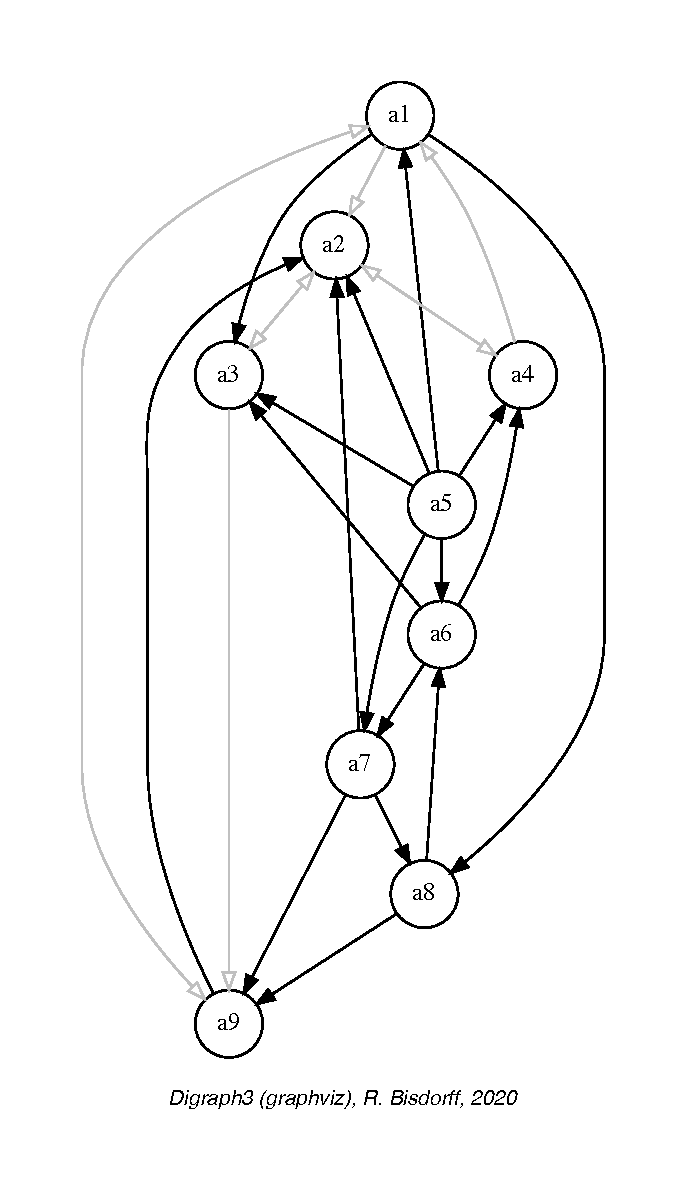
\includegraphics[width=7cm]{Figures/8-1-rankingTutorial.pdf}
\caption{The strict outranking relation $\succnsim$ shown here is, for instance, \emph{not transitive}: alternative \texttt{a8} outranks alternative \texttt{a6} and alternative \texttt{a6} outranks \texttt{a4}, however, \texttt{a8} does not outrank \texttt{a4}. Furthermore, alternatives \texttt{a6}, \texttt{a7} and \texttt{a8} show a cyclic outranking relation}
\label{fig:8.1}       % Give a unique label
\end{figure}

The \texttt{computeTransitivityDegree()} method\index{computeTransitivityDegree@\texttt{computeTransitivityDegree()}} computes the \emph{transitivity degree} of the outranking digraph shown in Figure~\vref{fig:8.1}, i.e. the ratio of the difference between the number of outranking arcs and the number of transitive arcs over the difference of the number of arcs of the transitive closure minus the transitive arcs of the digraph \texttt{gcd}.
\begin{lstlisting}
>>> gcd.computeTransitivityDegree(Comments=True)
 Transitivity degree of graph <codual_rel_randomCBperftab>
  triples x>y>z: 78, closed: 38, open: 40
  closed/triples = 0.487
\end{lstlisting}    

With only $49\%$ of the required transitive arcs, the strict outranking relation here is hence very far from being transitive; a serious problem when a linear ordering of the decision alternatives is looked for.

Let us furthermore check whether there are any cyclic outranking situations.
\begin{lstlisting}
>>> gcd.computeChordlessCircuits()
>>> gcd.showChordlessCircuits()
  1 circuit(s).
  *---- Chordless circuits ----*    
  1: ['a6', 'a7', 'a8'] , credibility : 0.033
\end{lstlisting}

There is one chordless circuit detected in the given strict outranking digraph \texttt{gcd}, namely alternative \texttt{a6} outranks alternative \texttt{a7}, the latter outranks \texttt{a8}, and \texttt{a8} outranks again alternative \texttt{a6} (see Fig.~\vref{fig:8.1}). Any potential linear ordering of these three alternatives will, in fact, always contradict somehow the given outranking relation.

Now, several heuristic ranking rules have been proposed for constructing a linear ordering which is closest in some specific sense to a given outranking relation. The \Digraph resources provide some of the most common of these ranking rules, like the \Copeland, \Kemeny, \Slater, \Kohler, and the \RankedPairs ranking rules.

\section{The \Copeland ranking}
\label{sec:8.2}

\begin{definition}[\Copeland ranking rule]\label{def:8.1}

\noindent The \Copeland ranking rule computes for each alternative a score resulting from the sum of the differences between the crisp \emph{strict outranking} characteristics $r(x\, \succnsim \,y)_{>0}$ and the crisp \emph{strict outranked} characteristics $r(y\, \succnsim \, x)_{>0}$  for all non-reflexive pairs of alternatives. The alternatives are ranked in decreasing order of these scores; ties, the case given, being resolved with a lexicographical rule applied to the identifiers of the alternatives \citep{COP-1951}.
\end{definition}

The \Copeland rule works well for any strict outranking relation which models a linear partial order on the \emph{median cut} strict outranking digraph \texttt{ccd} \citep{DIA-2010}. 
\begin{lstlisting}[caption={Computing a \Copeland Ranking},label=list:8.3]
>>> from linearOrders import CopelandRanking
>>> cop = CopelandRanking(gcd,Comments=True)
 Copeland decreasing scores
     a5 : +12
     a1 :  +2
     a6 :  +2
     a7 :  +2
     a8 :   0
     a4 :  -3
     a9 :  -3
     a3 :  -5
     a2 :  -7
  Copeland Ranking:
  ['a5','a1','a6','a7','a8','a4','a9','a3','a2']
\end{lstlisting}

Alternative \texttt{a5} obtains here the best \Copeland score ($+12$), followed by alternatives \texttt{a1}, \texttt{a6} and \texttt{a7} with same score ($+2$); following the lexicographic rule, \texttt{a1} is hence ranked before \texttt{a6} and \texttt{a6} before \texttt{a7}. Same situation is observed for \texttt{a4} and \texttt{a9} with a score of $-3$ (see List.~\vref{list:8.3} Lines 4-12). The \Copeland ranking rule is in fact \emph{invariant} under the \emph{codual} transform (see Sec.~\ref{sec:2.6}) and renders a same linear order indifferently from digraphs \texttt{g} or \texttt{gcd} .

In Listing~\vref{list:8.4}, the \texttt{computeRankingCorrelation()} method\index{computeRankingCorrelation@\texttt{computeRankingCorrelation()}}, coupled with the \texttt{showCorrelation()} method, indicate the ordinal correlation of the \Copeland ranking result, shown in Listing~\vref{list:8.3} Line 14, with the given outranking digraph \texttt{g} (see Chap.~\ref{sec:16} and \citet{BIS-2012a}).
\begin{lstlisting}[caption={Checking the ordinal quality of the \Copeland ranking},label=list:8.4]
>>> corr = g.computeRankingCorrelation(cop.copelandRanking)
>>> g.showCorrelation(corr)
 Correlation indexes:
   Crisp ordinal correlation : +0.463
   Valued equivalalence      : +0.107
   Epistemic determination   :  0.230
\end{lstlisting}

With an epistemic determination level of $0.230$ (Line 6), the crisp ordinal correlation --\Kendall $\tau$-- index of $+463$ is in fact supported by $61.5\% (100.0 x (1.0 + 0.23)/2)$ of the criteria significance weights. Furthermore, the bipolar-valued \emph{relational equivalence} characteristics between the strict outranking relation and the \Copeland ranking equals $+0.107$, i.e. a \emph{majority} of $55.35\%$ of the criteria significance supports the relational equivalence between the given strict outranking relation and the \Copeland ranking (see Chap.~\ref{sec:16}).

The \Copeland scores, shown in Listing~\vref{list:8.3} deliver actually only a \emph{weak ranking}, i.e. a ranking with ties. This weak ranking may be constructed with the \texttt{WeakCopelandOrder} class \index{WeakCopelandOrder@\texttt{WeakCopelandOrder} class} from the \texttt{transitiveDigraphs} module.\index{transitiveDigraphs@\texttt{transitiveDigraphs} module}
\begin{lstlisting}[caption={Computing a weak \Copeland ranking},label=list:8.5]
>>> from transitiveDigraphs import WeakCopelandOrder
>>> wcop = WeakCopelandOrder(g)
>>> wcop.showRankingByChoosing()
 Ranking by Choosing and Rejecting
   1st ranked ['a5']
     2nd ranked ['a1', 'a6', 'a7']
       3rd ranked ['a8']
       3rd last ranked ['a4', 'a9']
     2nd last ranked ['a3']
   1st last ranked ['a2']
\end{lstlisting}

We recover in Listing~\vref{list:8.5}, the preorder delivered by the \Copeland scores (see Listing~\vref{list:8.3}). We may draw its corresponding skeleton\footnote{The skeleton of a transitive relation drops the transitivity induced arcs.}.
\begin{lstlisting}
>>> wcop.exportGraphViz(fileName='weakCopelandRanking')
 *---- exporting a dot file for GraphViz tools ---------*
  Exporting to weakCopelandRanking.dot
  dot -Grankdir=TB -Tpng weakCopelandRanking.dot\
                   -o weakCopelandRanking.png
\end{lstlisting}
\begin{figure}[h]
\sidecaption[t]
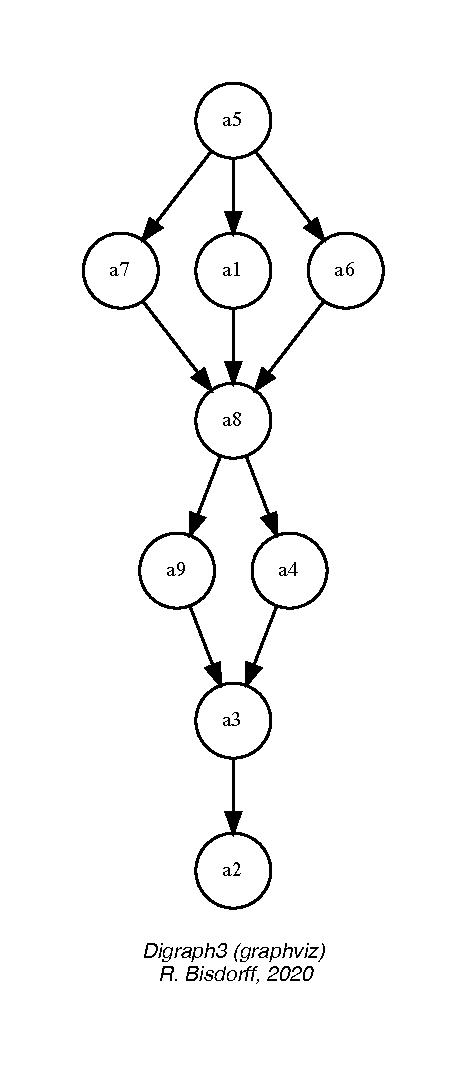
\includegraphics[width=5cm]{Figures/8-2-weakCopelandRanking.pdf}
\caption{Drawing of the weak \Copeland ranking. The graph show the skeleton of the preorder produced by the corresponding ties of the \Copeland scores}
\label{fig:8.2}       % Give a unique label
\end{figure}

Let us now consider a similar ranking rule, but working directly on the criteria \emph{significance majority margins}, i.e. the \emph{bipolar-valued} outranking relations.

\section{The \NetFlows ranking}
\label{sec:8.3}

\begin{definition}[\NetFlows ranking rule]\label{def:8.3}

\noindent The bipolar-valued version of the \Copeland ranking rule, we call \NetFlows \footnote{This ranking rule is also known under the name \Promethee ranking rule \citep*{BRA-1985}.}, computes for each alternative $x$ a \emph{net-flow} score,  i.e. the sum of the differences between the \emph{strict outranking} characteristics $r(x\, \succnsim \,y)$ and the \emph{strict outranked} characteristics $r(y\, \succnsim \,x)$ for all non-reflexive pairs of alternatives.
\end{definition}

The \texttt{NetFlowsRanking} class\index{NetFlowsRanking@\texttt{NetFlowsRanking} class} from the \texttt{linearOrders} module computes the \NetFlows ranking from a given outranking digraph.
\begin{lstlisting}[caption={Computing a \NetFlows ranking},label=list:8.6]
>>> from linearOrders import NetFlowsRanking
>>> nf = NetFlowsRanking(gcd,Comments=True)
  Net flow scores :
    a5 : +3.600
    a7 : +2.800
    a6 : +1.300
    a3 : +0.033
    a1 : -0.400
    a8 : -0.567
    a4 : -1.283
    a9 : -2.600
    a2 : -2.883
  NetFlows Ranking:
   ['a5','a7','a6','a3','a1','a8','a4','a9','a2']
>>> cop.copelandRanking # comparing both
   ['a5','a1','a6','a7','a8','a4','a9','a3','a2']
\end{lstlisting}

In our example here, the net-flows scores actually deliver a linear ranking \emph{without ties} which is rather different from the one delivered by the \Copeland rule (see List.~\vref{list:8.6} Line 16). It may happen, however, that we obtain, as with the \Copeland scores above, only a ranking with ties, which may then be resolved similarly by following a lexicographic rule applied to the identifiers of the decision alternatives. In such cases, it is possible to construct again a \emph{weak ranking} with the corresponding \texttt{WeakNetFlowsOrder} class\index{WeakNetFlowsOrder@\texttt{WeakNetFlowsOrder} class} from the \texttt{transitiveDigraphs} module.\index{transitiveDigraphs@\texttt{transitiveDigraphs} module}

It is worthwhile noticing again, that similar to the \Copeland ranking rule seen before, the \NetFlows ranking rule is also \emph{invariant} under the codual transform (see Sec.~\ref{sec:2.6}) and delivers again the same ranking result indifferently from digraphs \texttt{g} or \texttt{gcd} (see List.~\vref{list:8.6} Line 14). 

The \NetFlows ranking result appears to be slightly better correlated ($+0.638$) with the given strict outranking relation than its crisp cousin, the \Copeland ranking (see Lines 4-6 in List.~\vref{list:8.7}).
\begin{lstlisting}[caption={Checking the quality of the \NetFlows Ranking},label=list:8.7]   
>>> corr = gcd.computeOrdinalCorrelation(nf)
>>> gcd.showCorrelation(corr)
 Correlation indexes:
   Extended Kendall tau       : +0.638
   Epistemic determination    :  0.230
   Bipolar-valued equivalence : +0.147
\end{lstlisting}

Indeed, the ordinal correlation index of $+0.638$ leads to a bipolar-valued \emph{relational equivalence} characteristics of $+0.147$, i.e. a majority of $57.35\%$ of the criteria significance supports the relational equivalence between the given outranking digraphs $g$ or $gcd$  and the corresponding \NetFlows ranking (see Chap.~\ref{sec:16}). The weaker ordinal ranking quality of the \Copeland rule ($+0.463$) stems in this example here essentially from the \emph{weakness} of the actual \Copeland ranking result and our subsequent \emph{arbitrary} lexicographic resolution of the many ties given by the \Copeland scores (see Fig.~\vref{fig:8.2}).

To appreciate now the ordinal correlations of both the \Copeland and the \NetFlows rankings with the underlying strict outranking relation, it is useful to consider the '\emph{optimal}' \Kemeny and \Slater ranking rules.

\section{\Kemeny rankings}
\label{sec:8.4}

\begin{definition}[\Kemeny ranking rule]\label{def:8.3}

  \noindent A \Kemeny ranking $k$ is a linear ranking without ties of the set of $n$ decision alternatives $X$ which is \emph{closest}, in the sense of the ordinal \Kendall distance (see Chap.~\ref{sec:16} and \citet{BIS-2012b}), to the given valued outranking digraphs \texttt{g} \citep{KEM-1959}. Formally:
  \begin{equation}\label{eq:8.1}
    k \;=\; \text{argmax}_{p \in \mathcal{P}(X)} \sum_{i \neq j}\big(r(p[i] \succsim p[j]) - r(p[j] \succsim p[i]) \big),
  \end{equation}
where $\mathcal{P}(X)$ denotes the set of all permutations of $X$ and $i,j = 0,... n$.
\end{definition}

The \texttt{KemenyRanking} class\index{KemenyRanking@\texttt{KemenyRanking} class} from the \texttt{linearOrders} module computes such a ranking which is highest possible correlated with the underlying strict outranking relation. The \Kemeny rule is also \emph{invariant} under the codual transform.

Mind that the \texttt{KemenyRanking} class constructor, in order to find a \Kemeny ranking, has to compute a net-flows score for every permutation of the list of decision alternatives (see Eq.~\vref{eq:8.1}). Therefore the class is limited, by default, to digraphs of order up to 7 \citep{BIS-2021b}. In Listing~\vref{list:8.8} Line 2, the \texttt{orderLimit} parameter allows to rise this limit.
\begin{lstlisting}[caption={Computing a \Kemeny ranking},label=list:8.8]   
>>> from linearOrders import KemenyRanking
>>> ke = KemenyRanking(gcd,orderLimit=9)
>>> # default orderLimit is 7
>>> ke.showRanking()
 ['a5','a6','a7','a3','a9','a4','a1','a8','a2']
>>> corr = gcd.computeOrdinalCorrelation(ke)
>>> gcd.showCorrelation(corr)
 Correlation indexes:
   Extended Kendall tau       : +0.779
   Epistemic determination    :  0.230
   Bipolar-valued equivalence : +0.179
\end{lstlisting}    

So, $+0.779$ represents the \emph{highest possible} ordinal correlation index --\emph{fitness}-- any potential linear ranking can achieve with the given pairwise outranking digraph (see List.~\vref{list:8.8} Lines 8-11).

A \Kemeny ranking may not be unique. In our example here, we obtain in fact two such \Kemeny rankings with a same \emph{maximal} \Kemeny index of $12.92$. 
\begin{lstlisting}[caption={Optimal \Kemeny rankings},label=list:8.9]
>>> ke.maximalRankings
  [['a5','a6','a7','a3','a8','a9','a4','a1','a2'],
   ['a5','a6','a7','a3','a9','a4','a1','a8','a2']]
>>> ke.maxKemenyIndex
  Decimal('12.9166667')
\end{lstlisting}

We may visualise in Figure~\vref{fig:8.3} the partial order defined by the epistemic disjunction of both optimal \Kemeny rankings by using the \texttt{RankingsFu\-sion} class\index{RankingsFusion@\texttt{RankingsFusion} class} (see Sec.~\ref{sec:2.5}).
\begin{lstlisting}[caption={Computing the epistemic disjunction of all optimal \Kemeny rankings},label=list:8.9]   
>>> from transitiveDigraphs import RankingsFusion
>>> wke = RankingsFusion(ke,ke.maximalRankings)
>>> wke.exportGraphViz(fileName='tutorialKemeny')
 *---- exporting a dot file for GraphViz tools ---------*
  Exporting to tutorialKemeny.dot
  dot -Grankdir=TB -Tpng tutorialKemeny.dot -o tutorialKemeny.png
\end{lstlisting}
\begin{figure}[ht]
\sidecaption[t]
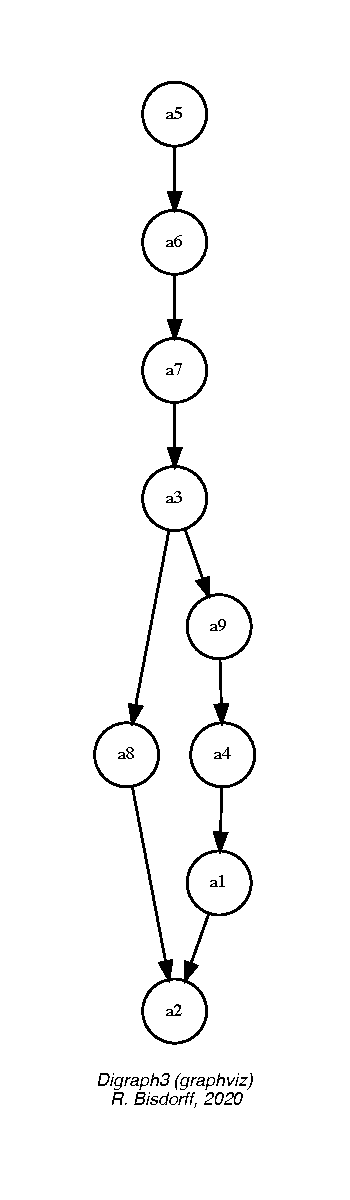
\includegraphics[width=5cm]{Figures/8-3-tutorialKemeny.pdf}
\caption{Epistemic disjunction of optimal \Kemeny rankings. It is interesting to notice that both \Kemeny rankings only differ in their respective positioning of alternative \texttt{a8}; either before or after alternatives \texttt{a9}, \texttt{a4} and \texttt{a1}}
\label{fig:8.3}       % Give a unique label
\end{figure}

To retain now a specific representative among all the potential rankings with maximal \Kemeny index, we will choose, with the help of the \texttt{showRankingCon\-sensusQuality()} method\index{showRankingConsensusQuality@Showrankingconsensusquality()}, the one proposing the best criteria consensus.
\begin{lstlisting}[caption={Computing the consensus quality of a ranking},label=list:8.10]   
>>> g.showRankingConsensusQuality(ke.maximalRankings[0])
 Consensus quality of ranking:
  ['a5','a6','a7','a3','a8','a9','a4','a1','a2']
  criterion (weight): correlation
  -------------------------------
      b09 (0.050)  : +0.361
      b04 (0.050)  : +0.333
      b08 (0.050)  : +0.292
      b01 (0.050)  : +0.264
      c01 (0.167)  : +0.250
      b03 (0.050)  : +0.222
      b07 (0.050)  : +0.194
      b05 (0.050)  : +0.167
      c02 (0.167)  : +0.000
      b10 (0.050)  : +0.000
      b02 (0.050)  : -0.042
      b06 (0.050)  : -0.097
      c03 (0.167)  : -0.167
  Summary:
    Weighted mean marginal correlation (a): +0.099
    Standard deviation (b)                : +0.177
    Ranking fairness (a)-(b)              : -0.079
>>> g.showRankingConsensusQuality(ke.maximalRankings[1])
 Consensus quality of ranking:
  ['a5','a6','a7','a3','a9','a4','a1','a8','a2']
  criterion (weight): correlation
  -------------------------------
      b09 (0.050)   : +0.306
      b08 (0.050)   : +0.236
      c01 (0.167)   : +0.194
      b07 (0.050)   : +0.194
      c02 (0.167)   : +0.167
      b04 (0.050)   : +0.167
      b03 (0.050)   : +0.167
      b01 (0.050)   : +0.153
      b05 (0.050)   : +0.056
      b02 (0.050)   : +0.014
      b06 (0.050)   : -0.042
      c03 (0.167)   : -0.111
      b10 (0.050)   : -0.111
  Summary:
    Weighted mean marginal correlation (a): +0.099
    Standard deviation (b)                : +0.132
    Ranking fairness (a)-(b)              : -0.033
\end{lstlisting}

Both \Kemeny rankings show the same \emph{weighted mean marginal correlation}: $+0.099$ with all thirteen performance criteria. However, the second ranking shows a slightly lower \emph{standard deviation}: $+0.132$ versus $+0.177$, resulting in a slightly \emph{fairer} ranking result: $-0.033$ versus $-0.079$ (see Listing~\vref{list:8.10} Lines 20-23, 42-44) .

When several rankings with maximal \Kemeny index are given, the \texttt{Kemeny\-Ranking} class constructor instantiates the ranking with \emph{highest} mean marginal correlation and, in case of ties, with \emph{lowest} weighted standard deviation. Here we obtain ranking: [\texttt{a5}, \texttt{a6}, \texttt{a7}, \texttt{a3}, \texttt{a9}, \texttt{a4}, \texttt{a1}, \texttt{a8}, \texttt{a2}] (see Line 4 in Listing~\vref{list:8.8} above).

\section{\Slater rankings}
\label{sec:8.5}

The \Slater ranking rule is identical to the \Kemeny rule, but it is working, instead, on the \Condorcet --\emph{median cut polarised}-- digraph \texttt{ccd} \citep{SLA-1961}. The \Slater rule is again \emph{invariant} under the codual transform and delivers hence indifferently on \texttt{g} or \texttt{gcd} the following results:
\begin{lstlisting}[caption={Computing a \Slater ranking},label=list:8.11]   
>>> from linearOrders import SlaterRanking
>>> sl = SlaterRanking(gcd,orderLimit=9)
>>> sl.slaterRanking
  ['a5','a6','a4','a1','a3','a7','a8','a9','a2']
>>> corr = gcd.computeRankingCorrelation(sl.slaterRanking)
>>> sl.showCorrelation(corr)
  Correlation indexes:
   Extended Kendall tau       : +0.676
   Epistemic determination    :  0.230
   Bipolar-valued equivalence : +0.156
>>> len(sl.maximalRankings)
  7
\end{lstlisting}

We notice in Listing~\vref{list:8.11} that the \Slater ranking shown in Line 4 represents a rather good fit ($+0.676$), slightly better apparently than the \NetFlows ranking result ($+0.638$). However, there are in fact 7 such optimal \Slater rankings (see Line 12). The corresponding epistemic disjunction gives the partial ordering shown in Fig~\vref{fig:8.4}:
\begin{lstlisting}[caption={Computing the epistemic disjunction of optimal \Slater rankings},label=list:8.12]   
>>> slw = RankingsFusion(sl,sl.maximalRankings)
>>> slw.exportGraphViz(fileName='tutorialSlater')
 *---- exporting a dot file for GraphViz tools ----*
  Exporting to tutorialSlater.dot
  dot -Grankdir=TB -Tpng tutorialSlater.dot\
                   -o tutorialSlater.png
\end{lstlisting}
\begin{figure}[ht]
\sidecaption[t]
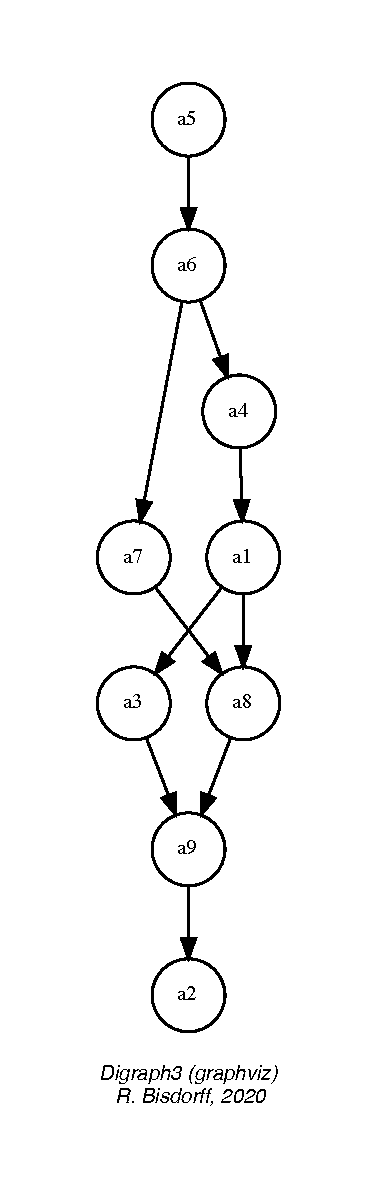
\includegraphics[width=5cm]{Figures/8-4-tutorialSlater.pdf}
\caption{Epistemic disjunction of optimal \Slater rankings. What precise \Slater ranking result should we hence adopt?}
\label{fig:8.4}       % Give a unique label
\end{figure}
       
The \Kemeny and \Slater ranking rules are furthermore computationally \emph{difficult} problems and effective ranking results are only computable for tiny outranking digraphs ($< 20$ objects) (see Eq.~\vref{eq:8.1}). 

More computationally efficient ranking heuristics, like the \Copeland and \NetFlows rules, are therefore needed in practice. Let us finally, after these \emph{ranking-by-scoring} strategies, also present two popular \emph{ranking-by-choosing} strategies.

\section{The \Kohler ranking-by-choosing rule}
\label{sec:8.6}

\begin{definition}[The \Kohler \emph{ranking-by-choosing} rule]\label{def:8.4}
  
\noindent At step $i$ ($i$ goes from 1 to $n$) do the following:
\begin{enumerate}[leftmargin=0.5cm,rightmargin=0.5cm,topsep=1pt]
\item Compute for each row of the bipolar-valued \emph{strict} outranking relation table (see Listing~\vref{list:8.1}) the smallest value;
\item Select the row where this minimum is maximal. Ties are resolved in lexicographic order;
\item Put the selected decision alternative at rank $i$;
\item Delete the corresponding row and column from the relation table and restart until the table is empty.
\end{enumerate}
\end{definition}
\begin{lstlisting}[caption={Computing a \Kohler ranking},label=list:8.13]   
>>> from linearOrders import KohlerRanking
>>> kocd = KohlerRanking(gcd)
>>> kocd.showRanking()
  ['a5','a7','a6','a3','a9','a8','a4','a1','a2']
>>> corr = gcd.computeOrdinalCorrelation(kocd)
>>> gcd.showCorrelation(corr)
  Correlation indexes:
    Extended Kendall tau       : +0.747
    Epistemic determination    :  0.230
    Bipolar-valued equivalence : +0.172
\end{lstlisting}

With this \emph{min-max} lexicographic ranking-by-choosing strategy, we find a correlation result ($+0.747$) that is until now clearly the nearest to an optimal \Kemeny ranking (see Listing~\vref{list:8.8}). Only two adjacent pairs: (\texttt{a6}, \texttt{a7}) and (\texttt{a8}, \texttt{a9}) are actually inverted here. Notice that the \Kohler ranking rule, contrary to the previously mentioned rules, is \textbf{not} invariant under the codual transform and requires to work on the \texttt{strict} outranking digraph \texttt{gcd} for a better correlation result.
\begin{lstlisting}
>>> ko = KohlerRanking(g)  
>>> corr = g.computeOrdinalCorrelation(ko)
>>> g.showCorrelation(corr)
  Correlation indexes:
   Crisp ordinal correlation  : +0.483
   Epistemic determination    :  0.230
   Bipolar-valued equivalence : +0.111
\end{lstlisting}

But the \Kohler rule has a \emph{dual} version, the prudent \emph{Arrow-Raynaud} ordering-by-choosing rule, where a corresponding \emph{max-min} strategy, when used on the \emph{non-strict} outranking digraph $g$, for ordering from \emph{last} to \emph{first} produces a similar ranking result \citep{ARR-1986}.

Noticing that the \NetFlows score of an alternative $x$ represents in fact a bipolar-valued characteristic of the assertion ``\emph{alternative x is ranked first}'', we may enhance the \Kohler rule by replacing the simple \emph{min-max} strategy with an \emph{iterated} maximal \NetFlows score selection.

\begin{definition}[The iterated \NetFlows ranking-by-choosing rule]
  
\noindent At step $i$ ($i$ goes from 1 to $n$) do the following:
\begin{enumerate}[leftmargin=0.5cm,rightmargin=0.5cm,topsep=1pt]
\item Compute for each row of the bipolar-valued outranking relation table (see Listing~\vref{list:8.1}) the corresponding \NetFlows score;
\item Select the row where this score is \emph{maximal}, ties being resolved by lexicographic order;
\item Put the corresponding decision alternative at rank $i$;
\item Delete the corresponding row and column from the relation table and restart until the table is empty.
\end{enumerate}
\end{definition}

The \texttt{IteratedNetFlowsRanking}\index{IteratedNetFlowsRanking@\texttt{IteratedNetFlowsRanking} class} class from the \texttt{linearOrders} module computes this ranking result. 
\begin{lstlisting}[caption={Ranking-by-choosing with iterated maximal \NetFlows scores},label=list:8.14]   
>>> from linearOrders import IteratedNetFlowsRanking  
>>> inf = IteratedNetFlowsRanking(g)
>>> inf
 *------- Digraph instance description ------*
   Instance class      : IteratedNetFlowsRanking
   Instance name       : rel_randomCBperftab_ranked
   Digraph Order       : 9
   Digraph Size        : 36
   Valuation domain    : [-1.00;1.00]
   Determinateness (%) : 100.00
   Attributes     : ['valuedRanks', 'valuedOrdering',
                     'iteratedNetFlowsRanking',
                     'iteratedNetFlowsOrdering',
                     'name', 'actions', 'order',
                     'valuationdomain', 'relation',
                     'gamma', 'notGamma']
>>> inf.iteratedNetFlowsRanking
  ['a5','a7','a6','a3','a4','a1','a8','a9','a2']
>>> corr = g.computeRankingCorrelation(\
...             inf.iteratedNetFlowsRanking)
>>> g.showCorrelation(corr)
  Correlation indexes:
    Crisp ordinal correlation  : +0.743
    Epistemic determination    :  0.230
    Bipolar-valued equivalence : +0.171
\end{lstlisting}

Like the \Kohler rule, the iterated \NetFlows rule has also a dual \emph{ordering-by-choosing} version, where instead of choosing at each step $i$ the row with maximal \NetFlows score, we choose the row with the \emph{minimal} \NetFlows score. Both the ranking and ordering result are computed by the \texttt{IteratedNetFlowsRanking} class (see Lines 12 and 13 in Listing~\vref{list:8.14}).
\begin{lstlisting}
>>> inf.iteratedNetFlowsOrdering
  ['a2','a9','a1','a4','a3','a8','a7','a6','a5']
>>> corr = g.computeOrderCorrelation(\
...                inf.iteratedNetFlowsOrdering)
>>> g.showCorrelation(corr)
  Correlation indexes:
    Crisp ordinal correlation  : +0.751
    Epistemic determination    : 0.230
    Bipolar-valued equivalence : +0.173
\end{lstlisting}

The iterated \NetFlows ranking and its dual, the iterated \NetFlows ordering, do not usually deliver both the same result. With our example outranking digraph $g$ for instance, it is the \emph{ordering-by-choosing} result who obtains a slightly better correlation with the given outranking digraph ($+0.751$), a result that is also slightly better than the original \Kohler ranking result ($+0.747$, see Listing~\vref{list:8.13} Line 8).

With different \emph{ranking-by-choosing} and \emph{ordering-by-choosing} results, it may be useful to \emph{fuse} now, similar to what we have done before with \Kemeny 's and \Slater 's optimal rankings, both, the iterated \NetFlows ranking and ordering into a partial ranking. But we are hence back to the practical problem of what linear ranking should we eventually retain? 

Let us finally mention another interesting \emph{ranking-by-choosing} approach.

\section{The \RankedPairs ranking rule}
\label{sec:8.7}

\emph{N. Tideman}'s \index{Tideman@\emph{Tideman}} ranking-by-choosing heuristic, the \RankedPairs rule, working best this time on the non strict outranking digraph $g$, is based on a \emph{prudent incremental} construction of linear orders that avoids on the fly any cycling outranking situations \citep{TID-1987}.

\begin{definition}[The \RankedPairs ranking rule]\label{def:8.5}
\begin{enumerate}[leftmargin=0.5cm,rightmargin=0.5cm,topsep=1pt]
 \item Rank the ordered pairs $(x,y)$ of alternatives in decreasing order of $r(x\, \succsim \,y) \,+\, r(y\, \not\succsim \,x)$;
 \item Consider the pairs in that order (ties are resolved by a lexicographic rule):
   \begin{itemize}[nosep]
     \item if the next pair does not create a \emph{circuit} with the pairs already blocked, block this pair;
     \item if the next pair creates a \emph{circuit} with the already blocked pairs, skip it.
    \end{itemize}
\end{enumerate}
\end{definition}  

With our didactic outranking digraph $g$, we get the following result.\index{RankedPairsRanking@\texttt{RankedPairsRanking} class}
\begin{lstlisting}[caption={Computing a \RankedPairs ranking},label=list:8.15]   
>>> from linearOrders import RankedPairsRanking
>>> rp = RankedPairsRanking(g)
>>> rp.showRanking()
  ['a5','a6','a7','a3','a8','a9','a4','a1','a2']
\end{lstlisting}

The \RankedPairs rule renders in our example here luckily one of the two optimal \Kemeny ranking, as we may verify below.
 \begin{lstlisting}
>>> ke.maximalRankings
  [['a5','a6','a7','a3','a8','a9','a4','a1','a2'],
   ['a5','a6','a7','a3','a9','a4','a1','a8','a2']]
>>> corr = g.computeOrdinalCorrelation(rp)
>>> g.showCorrelation(corr)
  Correlation indexes:
    Extended Kendall tau       : +0.779
    Epistemic determination    :  0.230
    Bipolar-valued equivalence : +0.179
\end{lstlisting}

Similar to \Kohler 's rule, the \RankedPairs rule has also a prudent dual version, the \emph{Dias-Lamboray} \emph{ordering-by-choosing} rule, which produces, when working this time on the codual strict outranking digraph gcd, a similar ranking result (see \citet*{LAM-2009,DIA-2010}).

Besides of not providing a unique linear ranking, the \emph{ranking-by-choosing} rules, as well as their duals, the \emph{ordering-by-choosing} rules, are unfortunately not scalable to outranking digraphs of larger orders ($> 100$). For such bigger outranking digraphs, with several hundred or thousands of alternatives, only the \Copeland and the \NetFlows \emph{ranking-by-scoring} rules, with a polynomial complexity of $\mathcal{O}(n^2)$, where $n$ is the order of the outranking digraph, remain in fact tractable. Furthermore, as computing the \Copeland and \NetFlows scores may be done separately per alternative, the latter ranking rules can right away be processed in parallel when multiprocessing resources are available.

\vspace{1cm}
The physical necessity to write down a list of items in a linear sequence renders the ranking decision problem very important in practice. However, a relative rating of such items into performance quantiles classes would be, from the very preference modelling perspective, more expressive and faithful. This is the subject of the following Chapter~\ref{sec:10}.


%%%%%%% The chapter bibliography
%\normallatexbib
\clearpage
%\phantomsection
%\addcontentsline{toc}{section}{References}
%\chapter{Ranking with multiple incommensurable criteria}
\label{sec:8}

\abstract*{ The \Digraph python resources provide several algorithms for solving the multiple incommensurable criteria ranking problem via bipolar-valued outranking digraphs. The \Copeland, \NetFlows, \Kemeny, \Slater, \Kohler, and the \RankedPairs ranking rules are introduced and illustrated with a random outranking digraph instance.}

\begin{quotation}''... \emph{whether we are deciding between buying different commodity baskets, or making choices about what to do on a holiday, or deciding for whom to vote for in an election, we are inescapably involved in evaluating alternatives with non–commensurable aspects}.''

  --\emph{Amartya Sen}, Idea of Justice, \citep{SEN-2009}\index{Sen@\emph{A. Sen}}
\end{quotation}
\vspace{1cm}

\abstract{The \Digraph python resources provide several algorithms for solving the multiple incommensurable criteria ranking problem via bipolar-valued outranking digraphs. The \Copeland, \NetFlows, \Kemeny, \Slater, \Kohler, and the \RankedPairs ranking rules are introduced and illustrated with a random outranking digraph.}

\section{The ranking problem}
\label{sec:8.1}

We need to rank without ties a set $X$ of items (usually decision alternatives) that are evaluated on multiple incommensurable performance criteria; yet, for which we may know their pairwise bipolar-valued \emph{strict outranking} characteristics, i.e. $r(x\, \succnsim \, y)$ for all $x, y \in X$ (see Sec.~\ref{sec:3.5} and \citep{BIS-2013}).

Let us consider in Listing~\vref{list:8.1} a didactic outranking digraph \texttt{g} generated from a random \emph{Cost-Benefit} performance tableau (see Sec.~\ref{sec:6.3}) concerning 9 decision alternatives evaluated on 13 performance criteria. We can compute the corresponding \emph{strict outranking digraph} with a codual transform (see Sec. ~\ref{sec:2.6}).
\begin{lstlisting}[caption={Random bipolar-valued strict outranking relation characteristics},label=list:8.1]
>>> from randomPerfTabs import RandomCBPerformanceTableau   
>>> t = RandomCBPerformanceTableau(numberOfActions=9,\
...         numberOfCriteria=13,seed=200)
>>> from outrankingDigraphs import BipolarOutrankingDigraph
>>> g = BipolarOutrankingDigraph(t)
>>> gcd = ~(-g) # codual digraph
>>> gcd.showRelationTable(ReflexiveTerms=False)
 * ---- Relation Table -----
  r(>) |  'a1'  'a2'  'a3'  'a4'  'a5'  'a6'  'a7'  'a8'  'a9'   
  -----|------------------------------------------------------
  'a1' |    -   0.00 +0.10 -1.00 -0.13 -0.57 -0.23 +0.10 +0.00  
  'a2' | -1.00   -    0.00 +0.00 -0.37 -0.42 -0.28 -0.32 -0.12  
  'a3' | -0.10  0.00   -   -0.17 -0.35 -0.30 -0.17 -0.17 +0.00  
  'a4' |  0.00  0.00 -0.42   -   -0.40 -0.20 -0.60 -0.27 -0.30  
  'a5' | +0.13 +0.22 +0.10 +0.40   -   +0.03 +0.40 -0.03 -0.07  
  'a6' | -0.07 -0.22 +0.20 +0.20 -0.37   -   +0.10 -0.03 -0.07  
  'a7' | -0.20 +0.28 -0.03 -0.07 -0.40 -0.10   -   +0.27 +1.00  
  'a8' | -0.10 -0.02 -0.23 -0.13 -0.37 +0.03 -0.27   -   +0.03  
  'a9' |  0.00 +0.12 -1.00 -0.13 -0.03 -0.03 -1.00 -0.03   -   
\end{lstlisting}
  
Some ranking rules will work on the associated \Condorcet digraph\index{Condorcet digraph}, i.e. the corresponding \emph{median cut} polarised strict outranking digraph.
 \begin{lstlisting}[caption={Median cut polarised strict outranking relation characteristics},label=list:8.2]
>>> ccd = PolarisedOutrankingDigraph(gcd,\
...                   level=g.valuationdomain['med'],\
...                   KeepValues=False,StrictCut=True)
>>> ccd.showRelationTable(ReflexiveTerms=False,\
...                       IntegerValues=True)
 *---- Relation Table -----
  r(>)_med | 'a1' 'a2' 'a3' 'a4' 'a5' 'a6' 'a7' 'a8' 'a9'   
  ---------|---------------------------------------------
     'a1'  |   -    0   +1   -1   -1   -1   -1   +1    0  
     'a2'  |  -1    -   +0    0   -1   -1   -1   -1   -1  
     'a3'  |  -1    0    -   -1   -1   -1   -1   -1    0  
     'a4'  |   0    0   -1    -   -1   -1   -1   -1   -1  
     'a5'  |  +1   +1   +1   +1    -   +1   +1   -1   -1  
     'a6'  |  -1   -1   +1   +1   -1    -   +1   -1   -1  
     'a7'  |  -1   +1   -1   -1   -1   -1    -   +1   +1  
     'a8'  |  -1   -1   -1   -1   -1   +1   -1    -   +1  
     'a9'  |   0   +1   -1   -1   -1   -1   -1   -1    -   
\end{lstlisting}

Unfortunately, such crisp median-cut \Condorcet digraphs, associated with a given strict outranking digraph, only exceptionally model a linear ordering. Usually, pairwise majority comparisons do not render a \emph{complete} or, at least, a \emph{transitive} partial order. There may even frequently appear \emph{cyclic} outranking situations (see Sec.~\ref{sec:7.4}).

To discover how \emph{difficult} this ranking problem can get, let us have a look in Figure.~\vref{fig:8.1} at the corresponding strict outranking digraph \emph{graphviz} drawing \footnote{ The \texttt{exportGraphViz()} method is depending on drawing tools from graphviz software (https://graphviz.org/).}.
\begin{lstlisting}
>>> gcd.exportGraphViz(fileName='rankingTutorial')
 *---- exporting a dot file for GraphViz tools ---------*
  Exporting to rankingTutorial.dot
  dot -Grankdir=BT -Tpng rankingTutorial.dot\
                   -o rankingTutorial.png
\end{lstlisting}
\begin{figure}[ht]
\sidecaption[t]
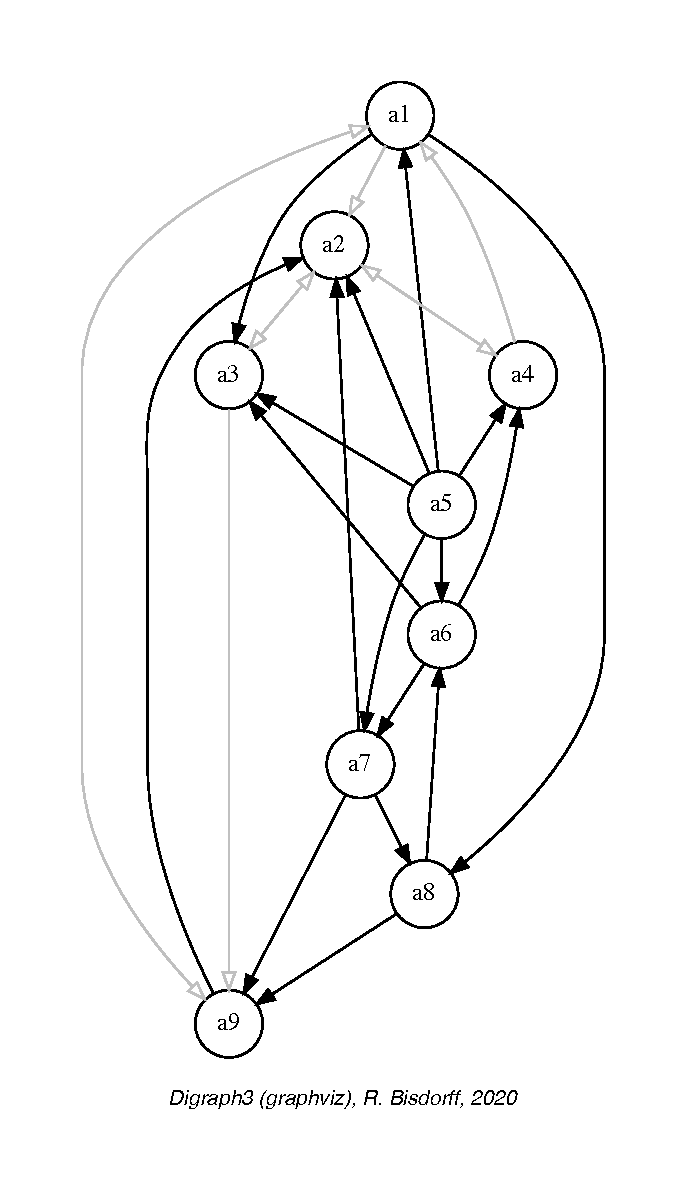
\includegraphics[width=7cm]{Figures/8-1-rankingTutorial.pdf}
\caption{The strict outranking relation $\succnsim$ shown here is, for instance, \emph{not transitive}: alternative \texttt{a8} outranks alternative \texttt{a6} and alternative \texttt{a6} outranks \texttt{a4}, however, \texttt{a8} does not outrank \texttt{a4}. Furthermore, alternatives \texttt{a6}, \texttt{a7} and \texttt{a8} show a cyclic outranking relation}
\label{fig:8.1}       % Give a unique label
\end{figure}

The \texttt{computeTransitivityDegree()} method\index{computeTransitivityDegree@\texttt{computeTransitivityDegree()}} computes the \emph{transitivity degree} of the outranking digraph shown in Figure~\vref{fig:8.1}, i.e. the ratio of the difference between the number of outranking arcs and the number of transitive arcs over the difference of the number of arcs of the transitive closure minus the transitive arcs of the digraph \texttt{gcd}.
\begin{lstlisting}
>>> gcd.computeTransitivityDegree(Comments=True)
 Transitivity degree of graph <codual_rel_randomCBperftab>
  triples x>y>z: 78, closed: 38, open: 40
  closed/triples = 0.487
\end{lstlisting}    

With only $49\%$ of the required transitive arcs, the strict outranking relation here is hence very far from being transitive; a serious problem when a linear ordering of the decision alternatives is looked for.

Let us furthermore check whether there are any cyclic outranking situations.
\begin{lstlisting}
>>> gcd.computeChordlessCircuits()
>>> gcd.showChordlessCircuits()
  1 circuit(s).
  *---- Chordless circuits ----*    
  1: ['a6', 'a7', 'a8'] , credibility : 0.033
\end{lstlisting}

There is one chordless circuit detected in the given strict outranking digraph \texttt{gcd}, namely alternative \texttt{a6} outranks alternative \texttt{a7}, the latter outranks \texttt{a8}, and \texttt{a8} outranks again alternative \texttt{a6} (see Fig.~\vref{fig:8.1}). Any potential linear ordering of these three alternatives will, in fact, always contradict somehow the given outranking relation.

Now, several heuristic ranking rules have been proposed for constructing a linear ordering which is closest in some specific sense to a given outranking relation. The \Digraph resources provide some of the most common of these ranking rules, like the \Copeland, \Kemeny, \Slater, \Kohler, and the \RankedPairs ranking rules.

\section{The \Copeland ranking}
\label{sec:8.2}

\begin{definition}[\Copeland ranking rule]\label{def:8.1}

\noindent The \Copeland ranking rule computes for each alternative a score resulting from the sum of the differences between the crisp \emph{strict outranking} characteristics $r(x\, \succnsim \,y)_{>0}$ and the crisp \emph{strict outranked} characteristics $r(y\, \succnsim \, x)_{>0}$  for all non-reflexive pairs of alternatives. The alternatives are ranked in decreasing order of these scores; ties, the case given, being resolved with a lexicographical rule applied to the identifiers of the alternatives \citep{COP-1951}.
\end{definition}

The \Copeland rule works well for any strict outranking relation which models a linear partial order on the \emph{median cut} strict outranking digraph \texttt{ccd} \citep{DIA-2010}. 
\begin{lstlisting}[caption={Computing a \Copeland Ranking},label=list:8.3]
>>> from linearOrders import CopelandRanking
>>> cop = CopelandRanking(gcd,Comments=True)
 Copeland decreasing scores
     a5 : +12
     a1 :  +2
     a6 :  +2
     a7 :  +2
     a8 :   0
     a4 :  -3
     a9 :  -3
     a3 :  -5
     a2 :  -7
  Copeland Ranking:
  ['a5','a1','a6','a7','a8','a4','a9','a3','a2']
\end{lstlisting}

Alternative \texttt{a5} obtains here the best \Copeland score ($+12$), followed by alternatives \texttt{a1}, \texttt{a6} and \texttt{a7} with same score ($+2$); following the lexicographic rule, \texttt{a1} is hence ranked before \texttt{a6} and \texttt{a6} before \texttt{a7}. Same situation is observed for \texttt{a4} and \texttt{a9} with a score of $-3$ (see List.~\vref{list:8.3} Lines 4-12). The \Copeland ranking rule is in fact \emph{invariant} under the \emph{codual} transform (see Sec.~\ref{sec:2.6}) and renders a same linear order indifferently from digraphs \texttt{g} or \texttt{gcd} .

In Listing~\vref{list:8.4}, the \texttt{computeRankingCorrelation()} method\index{computeRankingCorrelation@\texttt{computeRankingCorrelation()}}, coupled with the \texttt{showCorrelation()} method, indicate the ordinal correlation of the \Copeland ranking result, shown in Listing~\vref{list:8.3} Line 14, with the given outranking digraph \texttt{g} (see Chap.~\ref{sec:16} and \citet{BIS-2012a}).
\begin{lstlisting}[caption={Checking the ordinal quality of the \Copeland ranking},label=list:8.4]
>>> corr = g.computeRankingCorrelation(cop.copelandRanking)
>>> g.showCorrelation(corr)
 Correlation indexes:
   Crisp ordinal correlation : +0.463
   Valued equivalalence      : +0.107
   Epistemic determination   :  0.230
\end{lstlisting}

With an epistemic determination level of $0.230$ (Line 6), the crisp ordinal correlation --\Kendall $\tau$-- index of $+463$ is in fact supported by $61.5\% (100.0 x (1.0 + 0.23)/2)$ of the criteria significance weights. Furthermore, the bipolar-valued \emph{relational equivalence} characteristics between the strict outranking relation and the \Copeland ranking equals $+0.107$, i.e. a \emph{majority} of $55.35\%$ of the criteria significance supports the relational equivalence between the given strict outranking relation and the \Copeland ranking (see Chap.~\ref{sec:16}).

The \Copeland scores, shown in Listing~\vref{list:8.3} deliver actually only a \emph{weak ranking}, i.e. a ranking with ties. This weak ranking may be constructed with the \texttt{WeakCopelandOrder} class \index{WeakCopelandOrder@\texttt{WeakCopelandOrder} class} from the \texttt{transitiveDigraphs} module.\index{transitiveDigraphs@\texttt{transitiveDigraphs} module}
\begin{lstlisting}[caption={Computing a weak \Copeland ranking},label=list:8.5]
>>> from transitiveDigraphs import WeakCopelandOrder
>>> wcop = WeakCopelandOrder(g)
>>> wcop.showRankingByChoosing()
 Ranking by Choosing and Rejecting
   1st ranked ['a5']
     2nd ranked ['a1', 'a6', 'a7']
       3rd ranked ['a8']
       3rd last ranked ['a4', 'a9']
     2nd last ranked ['a3']
   1st last ranked ['a2']
\end{lstlisting}

We recover in Listing~\vref{list:8.5}, the preorder delivered by the \Copeland scores (see Listing~\vref{list:8.3}). We may draw its corresponding skeleton\footnote{The skeleton of a transitive relation drops the transitivity induced arcs.}.
\begin{lstlisting}
>>> wcop.exportGraphViz(fileName='weakCopelandRanking')
 *---- exporting a dot file for GraphViz tools ---------*
  Exporting to weakCopelandRanking.dot
  dot -Grankdir=TB -Tpng weakCopelandRanking.dot\
                   -o weakCopelandRanking.png
\end{lstlisting}
\begin{figure}[h]
\sidecaption[t]
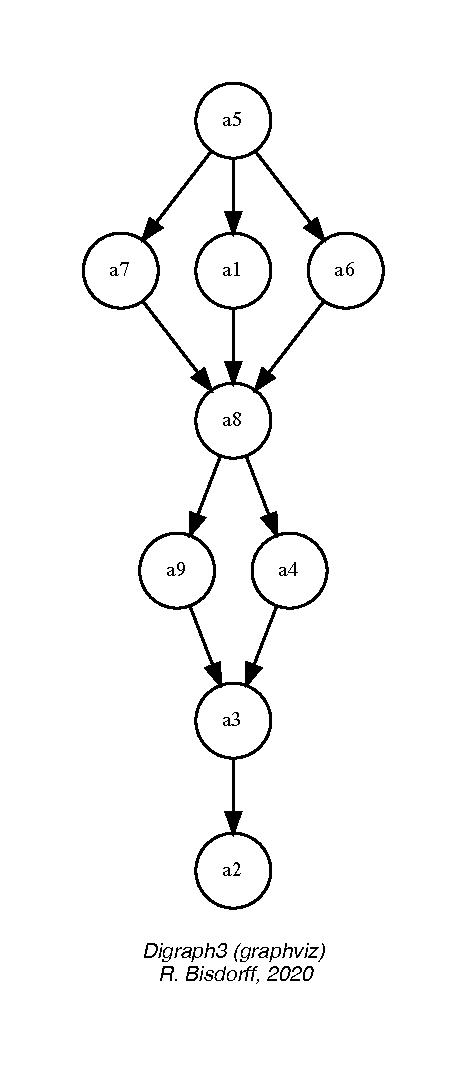
\includegraphics[width=5cm]{Figures/8-2-weakCopelandRanking.pdf}
\caption{Drawing of the weak \Copeland ranking. The graph show the skeleton of the preorder produced by the corresponding ties of the \Copeland scores}
\label{fig:8.2}       % Give a unique label
\end{figure}

Let us now consider a similar ranking rule, but working directly on the criteria \emph{significance majority margins}, i.e. the \emph{bipolar-valued} outranking relations.

\section{The \NetFlows ranking}
\label{sec:8.3}

\begin{definition}[\NetFlows ranking rule]\label{def:8.3}

\noindent The bipolar-valued version of the \Copeland ranking rule, we call \NetFlows \footnote{This ranking rule is also known under the name \Promethee ranking rule \citep*{BRA-1985}.}, computes for each alternative $x$ a \emph{net-flow} score,  i.e. the sum of the differences between the \emph{strict outranking} characteristics $r(x\, \succnsim \,y)$ and the \emph{strict outranked} characteristics $r(y\, \succnsim \,x)$ for all non-reflexive pairs of alternatives.
\end{definition}

The \texttt{NetFlowsRanking} class\index{NetFlowsRanking@\texttt{NetFlowsRanking} class} from the \texttt{linearOrders} module computes the \NetFlows ranking from a given outranking digraph.
\begin{lstlisting}[caption={Computing a \NetFlows ranking},label=list:8.6]
>>> from linearOrders import NetFlowsRanking
>>> nf = NetFlowsRanking(gcd,Comments=True)
  Net flow scores :
    a5 : +3.600
    a7 : +2.800
    a6 : +1.300
    a3 : +0.033
    a1 : -0.400
    a8 : -0.567
    a4 : -1.283
    a9 : -2.600
    a2 : -2.883
  NetFlows Ranking:
   ['a5','a7','a6','a3','a1','a8','a4','a9','a2']
>>> cop.copelandRanking # comparing both
   ['a5','a1','a6','a7','a8','a4','a9','a3','a2']
\end{lstlisting}

In our example here, the net-flows scores actually deliver a linear ranking \emph{without ties} which is rather different from the one delivered by the \Copeland rule (see List.~\vref{list:8.6} Line 16). It may happen, however, that we obtain, as with the \Copeland scores above, only a ranking with ties, which may then be resolved similarly by following a lexicographic rule applied to the identifiers of the decision alternatives. In such cases, it is possible to construct again a \emph{weak ranking} with the corresponding \texttt{WeakNetFlowsOrder} class\index{WeakNetFlowsOrder@\texttt{WeakNetFlowsOrder} class} from the \texttt{transitiveDigraphs} module.\index{transitiveDigraphs@\texttt{transitiveDigraphs} module}

It is worthwhile noticing again, that similar to the \Copeland ranking rule seen before, the \NetFlows ranking rule is also \emph{invariant} under the codual transform (see Sec.~\ref{sec:2.6}) and delivers again the same ranking result indifferently from digraphs \texttt{g} or \texttt{gcd} (see List.~\vref{list:8.6} Line 14). 

The \NetFlows ranking result appears to be slightly better correlated ($+0.638$) with the given strict outranking relation than its crisp cousin, the \Copeland ranking (see Lines 4-6 in List.~\vref{list:8.7}).
\begin{lstlisting}[caption={Checking the quality of the \NetFlows Ranking},label=list:8.7]   
>>> corr = gcd.computeOrdinalCorrelation(nf)
>>> gcd.showCorrelation(corr)
 Correlation indexes:
   Extended Kendall tau       : +0.638
   Epistemic determination    :  0.230
   Bipolar-valued equivalence : +0.147
\end{lstlisting}

Indeed, the ordinal correlation index of $+0.638$ leads to a bipolar-valued \emph{relational equivalence} characteristics of $+0.147$, i.e. a majority of $57.35\%$ of the criteria significance supports the relational equivalence between the given outranking digraphs $g$ or $gcd$  and the corresponding \NetFlows ranking (see Chap.~\ref{sec:16}). The weaker ordinal ranking quality of the \Copeland rule ($+0.463$) stems in this example here essentially from the \emph{weakness} of the actual \Copeland ranking result and our subsequent \emph{arbitrary} lexicographic resolution of the many ties given by the \Copeland scores (see Fig.~\vref{fig:8.2}).

To appreciate now the ordinal correlations of both the \Copeland and the \NetFlows rankings with the underlying strict outranking relation, it is useful to consider the '\emph{optimal}' \Kemeny and \Slater ranking rules.

\section{\Kemeny rankings}
\label{sec:8.4}

\begin{definition}[\Kemeny ranking rule]\label{def:8.3}

  \noindent A \Kemeny ranking $k$ is a linear ranking without ties of the set of $n$ decision alternatives $X$ which is \emph{closest}, in the sense of the ordinal \Kendall distance (see Chap.~\ref{sec:16} and \citet{BIS-2012b}), to the given valued outranking digraphs \texttt{g} \citep{KEM-1959}. Formally:
  \begin{equation}\label{eq:8.1}
    k \;=\; \text{argmax}_{p \in \mathcal{P}(X)} \sum_{i \neq j}\big(r(p[i] \succsim p[j]) - r(p[j] \succsim p[i]) \big),
  \end{equation}
where $\mathcal{P}(X)$ denotes the set of all permutations of $X$ and $i,j = 0,... n$.
\end{definition}

The \texttt{KemenyRanking} class\index{KemenyRanking@\texttt{KemenyRanking} class} from the \texttt{linearOrders} module computes such a ranking which is highest possible correlated with the underlying strict outranking relation. The \Kemeny rule is also \emph{invariant} under the codual transform.

Mind that the \texttt{KemenyRanking} class constructor, in order to find a \Kemeny ranking, has to compute a net-flows score for every permutation of the list of decision alternatives (see Eq.~\vref{eq:8.1}). Therefore the class is limited, by default, to digraphs of order up to 7 \citep{BIS-2021b}. In Listing~\vref{list:8.8} Line 2, the \texttt{orderLimit} parameter allows to rise this limit.
\begin{lstlisting}[caption={Computing a \Kemeny ranking},label=list:8.8]   
>>> from linearOrders import KemenyRanking
>>> ke = KemenyRanking(gcd,orderLimit=9)
>>> # default orderLimit is 7
>>> ke.showRanking()
 ['a5','a6','a7','a3','a9','a4','a1','a8','a2']
>>> corr = gcd.computeOrdinalCorrelation(ke)
>>> gcd.showCorrelation(corr)
 Correlation indexes:
   Extended Kendall tau       : +0.779
   Epistemic determination    :  0.230
   Bipolar-valued equivalence : +0.179
\end{lstlisting}    

So, $+0.779$ represents the \emph{highest possible} ordinal correlation index --\emph{fitness}-- any potential linear ranking can achieve with the given pairwise outranking digraph (see List.~\vref{list:8.8} Lines 8-11).

A \Kemeny ranking may not be unique. In our example here, we obtain in fact two such \Kemeny rankings with a same \emph{maximal} \Kemeny index of $12.92$. 
\begin{lstlisting}[caption={Optimal \Kemeny rankings},label=list:8.9]
>>> ke.maximalRankings
  [['a5','a6','a7','a3','a8','a9','a4','a1','a2'],
   ['a5','a6','a7','a3','a9','a4','a1','a8','a2']]
>>> ke.maxKemenyIndex
  Decimal('12.9166667')
\end{lstlisting}

We may visualise in Figure~\vref{fig:8.3} the partial order defined by the epistemic disjunction of both optimal \Kemeny rankings by using the \texttt{RankingsFu\-sion} class\index{RankingsFusion@\texttt{RankingsFusion} class} (see Sec.~\ref{sec:2.5}).
\begin{lstlisting}[caption={Computing the epistemic disjunction of all optimal \Kemeny rankings},label=list:8.9]   
>>> from transitiveDigraphs import RankingsFusion
>>> wke = RankingsFusion(ke,ke.maximalRankings)
>>> wke.exportGraphViz(fileName='tutorialKemeny')
 *---- exporting a dot file for GraphViz tools ---------*
  Exporting to tutorialKemeny.dot
  dot -Grankdir=TB -Tpng tutorialKemeny.dot -o tutorialKemeny.png
\end{lstlisting}
\begin{figure}[ht]
\sidecaption[t]
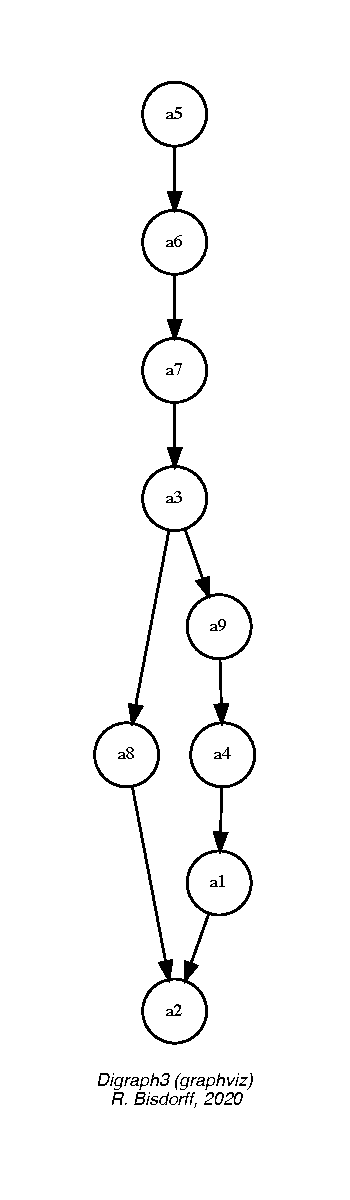
\includegraphics[width=5cm]{Figures/8-3-tutorialKemeny.pdf}
\caption{Epistemic disjunction of optimal \Kemeny rankings. It is interesting to notice that both \Kemeny rankings only differ in their respective positioning of alternative \texttt{a8}; either before or after alternatives \texttt{a9}, \texttt{a4} and \texttt{a1}}
\label{fig:8.3}       % Give a unique label
\end{figure}

To retain now a specific representative among all the potential rankings with maximal \Kemeny index, we will choose, with the help of the \texttt{showRankingCon\-sensusQuality()} method\index{showRankingConsensusQuality@Showrankingconsensusquality()}, the one proposing the best criteria consensus.
\begin{lstlisting}[caption={Computing the consensus quality of a ranking},label=list:8.10]   
>>> g.showRankingConsensusQuality(ke.maximalRankings[0])
 Consensus quality of ranking:
  ['a5','a6','a7','a3','a8','a9','a4','a1','a2']
  criterion (weight): correlation
  -------------------------------
      b09 (0.050)  : +0.361
      b04 (0.050)  : +0.333
      b08 (0.050)  : +0.292
      b01 (0.050)  : +0.264
      c01 (0.167)  : +0.250
      b03 (0.050)  : +0.222
      b07 (0.050)  : +0.194
      b05 (0.050)  : +0.167
      c02 (0.167)  : +0.000
      b10 (0.050)  : +0.000
      b02 (0.050)  : -0.042
      b06 (0.050)  : -0.097
      c03 (0.167)  : -0.167
  Summary:
    Weighted mean marginal correlation (a): +0.099
    Standard deviation (b)                : +0.177
    Ranking fairness (a)-(b)              : -0.079
>>> g.showRankingConsensusQuality(ke.maximalRankings[1])
 Consensus quality of ranking:
  ['a5','a6','a7','a3','a9','a4','a1','a8','a2']
  criterion (weight): correlation
  -------------------------------
      b09 (0.050)   : +0.306
      b08 (0.050)   : +0.236
      c01 (0.167)   : +0.194
      b07 (0.050)   : +0.194
      c02 (0.167)   : +0.167
      b04 (0.050)   : +0.167
      b03 (0.050)   : +0.167
      b01 (0.050)   : +0.153
      b05 (0.050)   : +0.056
      b02 (0.050)   : +0.014
      b06 (0.050)   : -0.042
      c03 (0.167)   : -0.111
      b10 (0.050)   : -0.111
  Summary:
    Weighted mean marginal correlation (a): +0.099
    Standard deviation (b)                : +0.132
    Ranking fairness (a)-(b)              : -0.033
\end{lstlisting}

Both \Kemeny rankings show the same \emph{weighted mean marginal correlation}: $+0.099$ with all thirteen performance criteria. However, the second ranking shows a slightly lower \emph{standard deviation}: $+0.132$ versus $+0.177$, resulting in a slightly \emph{fairer} ranking result: $-0.033$ versus $-0.079$ (see Listing~\vref{list:8.10} Lines 20-23, 42-44) .

When several rankings with maximal \Kemeny index are given, the \texttt{Kemeny\-Ranking} class constructor instantiates the ranking with \emph{highest} mean marginal correlation and, in case of ties, with \emph{lowest} weighted standard deviation. Here we obtain ranking: [\texttt{a5}, \texttt{a6}, \texttt{a7}, \texttt{a3}, \texttt{a9}, \texttt{a4}, \texttt{a1}, \texttt{a8}, \texttt{a2}] (see Line 4 in Listing~\vref{list:8.8} above).

\section{\Slater rankings}
\label{sec:8.5}

The \Slater ranking rule is identical to the \Kemeny rule, but it is working, instead, on the \Condorcet --\emph{median cut polarised}-- digraph \texttt{ccd} \citep{SLA-1961}. The \Slater rule is again \emph{invariant} under the codual transform and delivers hence indifferently on \texttt{g} or \texttt{gcd} the following results:
\begin{lstlisting}[caption={Computing a \Slater ranking},label=list:8.11]   
>>> from linearOrders import SlaterRanking
>>> sl = SlaterRanking(gcd,orderLimit=9)
>>> sl.slaterRanking
  ['a5','a6','a4','a1','a3','a7','a8','a9','a2']
>>> corr = gcd.computeRankingCorrelation(sl.slaterRanking)
>>> sl.showCorrelation(corr)
  Correlation indexes:
   Extended Kendall tau       : +0.676
   Epistemic determination    :  0.230
   Bipolar-valued equivalence : +0.156
>>> len(sl.maximalRankings)
  7
\end{lstlisting}

We notice in Listing~\vref{list:8.11} that the \Slater ranking shown in Line 4 represents a rather good fit ($+0.676$), slightly better apparently than the \NetFlows ranking result ($+0.638$). However, there are in fact 7 such optimal \Slater rankings (see Line 12). The corresponding epistemic disjunction gives the partial ordering shown in Fig~\vref{fig:8.4}:
\begin{lstlisting}[caption={Computing the epistemic disjunction of optimal \Slater rankings},label=list:8.12]   
>>> slw = RankingsFusion(sl,sl.maximalRankings)
>>> slw.exportGraphViz(fileName='tutorialSlater')
 *---- exporting a dot file for GraphViz tools ----*
  Exporting to tutorialSlater.dot
  dot -Grankdir=TB -Tpng tutorialSlater.dot\
                   -o tutorialSlater.png
\end{lstlisting}
\begin{figure}[ht]
\sidecaption[t]
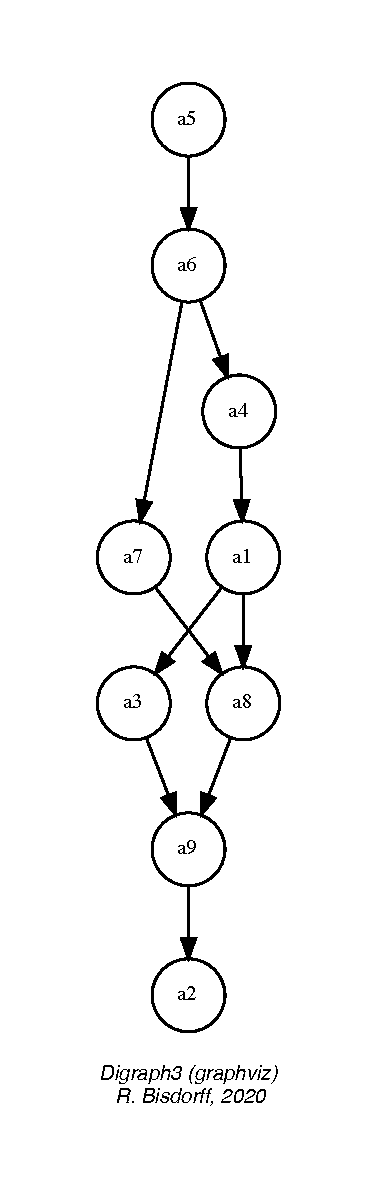
\includegraphics[width=5cm]{Figures/8-4-tutorialSlater.pdf}
\caption{Epistemic disjunction of optimal \Slater rankings. What precise \Slater ranking result should we hence adopt?}
\label{fig:8.4}       % Give a unique label
\end{figure}
       
The \Kemeny and \Slater ranking rules are furthermore computationally \emph{difficult} problems and effective ranking results are only computable for tiny outranking digraphs ($< 20$ objects) (see Eq.~\vref{eq:8.1}). 

More computationally efficient ranking heuristics, like the \Copeland and \NetFlows rules, are therefore needed in practice. Let us finally, after these \emph{ranking-by-scoring} strategies, also present two popular \emph{ranking-by-choosing} strategies.

\section{The \Kohler ranking-by-choosing rule}
\label{sec:8.6}

\begin{definition}[The \Kohler \emph{ranking-by-choosing} rule]\label{def:8.4}
  
\noindent At step $i$ ($i$ goes from 1 to $n$) do the following:
\begin{enumerate}[leftmargin=0.5cm,rightmargin=0.5cm,topsep=1pt]
\item Compute for each row of the bipolar-valued \emph{strict} outranking relation table (see Listing~\vref{list:8.1}) the smallest value;
\item Select the row where this minimum is maximal. Ties are resolved in lexicographic order;
\item Put the selected decision alternative at rank $i$;
\item Delete the corresponding row and column from the relation table and restart until the table is empty.
\end{enumerate}
\end{definition}
\begin{lstlisting}[caption={Computing a \Kohler ranking},label=list:8.13]   
>>> from linearOrders import KohlerRanking
>>> kocd = KohlerRanking(gcd)
>>> kocd.showRanking()
  ['a5','a7','a6','a3','a9','a8','a4','a1','a2']
>>> corr = gcd.computeOrdinalCorrelation(kocd)
>>> gcd.showCorrelation(corr)
  Correlation indexes:
    Extended Kendall tau       : +0.747
    Epistemic determination    :  0.230
    Bipolar-valued equivalence : +0.172
\end{lstlisting}

With this \emph{min-max} lexicographic ranking-by-choosing strategy, we find a correlation result ($+0.747$) that is until now clearly the nearest to an optimal \Kemeny ranking (see Listing~\vref{list:8.8}). Only two adjacent pairs: (\texttt{a6}, \texttt{a7}) and (\texttt{a8}, \texttt{a9}) are actually inverted here. Notice that the \Kohler ranking rule, contrary to the previously mentioned rules, is \textbf{not} invariant under the codual transform and requires to work on the \texttt{strict} outranking digraph \texttt{gcd} for a better correlation result.
\begin{lstlisting}
>>> ko = KohlerRanking(g)  
>>> corr = g.computeOrdinalCorrelation(ko)
>>> g.showCorrelation(corr)
  Correlation indexes:
   Crisp ordinal correlation  : +0.483
   Epistemic determination    :  0.230
   Bipolar-valued equivalence : +0.111
\end{lstlisting}

But the \Kohler rule has a \emph{dual} version, the prudent \emph{Arrow-Raynaud} ordering-by-choosing rule, where a corresponding \emph{max-min} strategy, when used on the \emph{non-strict} outranking digraph $g$, for ordering from \emph{last} to \emph{first} produces a similar ranking result \citep{ARR-1986}.

Noticing that the \NetFlows score of an alternative $x$ represents in fact a bipolar-valued characteristic of the assertion ``\emph{alternative x is ranked first}'', we may enhance the \Kohler rule by replacing the simple \emph{min-max} strategy with an \emph{iterated} maximal \NetFlows score selection.

\begin{definition}[The iterated \NetFlows ranking-by-choosing rule]
  
\noindent At step $i$ ($i$ goes from 1 to $n$) do the following:
\begin{enumerate}[leftmargin=0.5cm,rightmargin=0.5cm,topsep=1pt]
\item Compute for each row of the bipolar-valued outranking relation table (see Listing~\vref{list:8.1}) the corresponding \NetFlows score;
\item Select the row where this score is \emph{maximal}, ties being resolved by lexicographic order;
\item Put the corresponding decision alternative at rank $i$;
\item Delete the corresponding row and column from the relation table and restart until the table is empty.
\end{enumerate}
\end{definition}

The \texttt{IteratedNetFlowsRanking}\index{IteratedNetFlowsRanking@\texttt{IteratedNetFlowsRanking} class} class from the \texttt{linearOrders} module computes this ranking result. 
\begin{lstlisting}[caption={Ranking-by-choosing with iterated maximal \NetFlows scores},label=list:8.14]   
>>> from linearOrders import IteratedNetFlowsRanking  
>>> inf = IteratedNetFlowsRanking(g)
>>> inf
 *------- Digraph instance description ------*
   Instance class      : IteratedNetFlowsRanking
   Instance name       : rel_randomCBperftab_ranked
   Digraph Order       : 9
   Digraph Size        : 36
   Valuation domain    : [-1.00;1.00]
   Determinateness (%) : 100.00
   Attributes     : ['valuedRanks', 'valuedOrdering',
                     'iteratedNetFlowsRanking',
                     'iteratedNetFlowsOrdering',
                     'name', 'actions', 'order',
                     'valuationdomain', 'relation',
                     'gamma', 'notGamma']
>>> inf.iteratedNetFlowsRanking
  ['a5','a7','a6','a3','a4','a1','a8','a9','a2']
>>> corr = g.computeRankingCorrelation(\
...             inf.iteratedNetFlowsRanking)
>>> g.showCorrelation(corr)
  Correlation indexes:
    Crisp ordinal correlation  : +0.743
    Epistemic determination    :  0.230
    Bipolar-valued equivalence : +0.171
\end{lstlisting}

Like the \Kohler rule, the iterated \NetFlows rule has also a dual \emph{ordering-by-choosing} version, where instead of choosing at each step $i$ the row with maximal \NetFlows score, we choose the row with the \emph{minimal} \NetFlows score. Both the ranking and ordering result are computed by the \texttt{IteratedNetFlowsRanking} class (see Lines 12 and 13 in Listing~\vref{list:8.14}).
\begin{lstlisting}
>>> inf.iteratedNetFlowsOrdering
  ['a2','a9','a1','a4','a3','a8','a7','a6','a5']
>>> corr = g.computeOrderCorrelation(\
...                inf.iteratedNetFlowsOrdering)
>>> g.showCorrelation(corr)
  Correlation indexes:
    Crisp ordinal correlation  : +0.751
    Epistemic determination    : 0.230
    Bipolar-valued equivalence : +0.173
\end{lstlisting}

The iterated \NetFlows ranking and its dual, the iterated \NetFlows ordering, do not usually deliver both the same result. With our example outranking digraph $g$ for instance, it is the \emph{ordering-by-choosing} result who obtains a slightly better correlation with the given outranking digraph ($+0.751$), a result that is also slightly better than the original \Kohler ranking result ($+0.747$, see Listing~\vref{list:8.13} Line 8).

With different \emph{ranking-by-choosing} and \emph{ordering-by-choosing} results, it may be useful to \emph{fuse} now, similar to what we have done before with \Kemeny 's and \Slater 's optimal rankings, both, the iterated \NetFlows ranking and ordering into a partial ranking. But we are hence back to the practical problem of what linear ranking should we eventually retain? 

Let us finally mention another interesting \emph{ranking-by-choosing} approach.

\section{The \RankedPairs ranking rule}
\label{sec:8.7}

\emph{N. Tideman}'s \index{Tideman@\emph{Tideman}} ranking-by-choosing heuristic, the \RankedPairs rule, working best this time on the non strict outranking digraph $g$, is based on a \emph{prudent incremental} construction of linear orders that avoids on the fly any cycling outranking situations \citep{TID-1987}.

\begin{definition}[The \RankedPairs ranking rule]\label{def:8.5}
\begin{enumerate}[leftmargin=0.5cm,rightmargin=0.5cm,topsep=1pt]
 \item Rank the ordered pairs $(x,y)$ of alternatives in decreasing order of $r(x\, \succsim \,y) \,+\, r(y\, \not\succsim \,x)$;
 \item Consider the pairs in that order (ties are resolved by a lexicographic rule):
   \begin{itemize}[nosep]
     \item if the next pair does not create a \emph{circuit} with the pairs already blocked, block this pair;
     \item if the next pair creates a \emph{circuit} with the already blocked pairs, skip it.
    \end{itemize}
\end{enumerate}
\end{definition}  

With our didactic outranking digraph $g$, we get the following result.\index{RankedPairsRanking@\texttt{RankedPairsRanking} class}
\begin{lstlisting}[caption={Computing a \RankedPairs ranking},label=list:8.15]   
>>> from linearOrders import RankedPairsRanking
>>> rp = RankedPairsRanking(g)
>>> rp.showRanking()
  ['a5','a6','a7','a3','a8','a9','a4','a1','a2']
\end{lstlisting}

The \RankedPairs rule renders in our example here luckily one of the two optimal \Kemeny ranking, as we may verify below.
 \begin{lstlisting}
>>> ke.maximalRankings
  [['a5','a6','a7','a3','a8','a9','a4','a1','a2'],
   ['a5','a6','a7','a3','a9','a4','a1','a8','a2']]
>>> corr = g.computeOrdinalCorrelation(rp)
>>> g.showCorrelation(corr)
  Correlation indexes:
    Extended Kendall tau       : +0.779
    Epistemic determination    :  0.230
    Bipolar-valued equivalence : +0.179
\end{lstlisting}

Similar to \Kohler 's rule, the \RankedPairs rule has also a prudent dual version, the \emph{Dias-Lamboray} \emph{ordering-by-choosing} rule, which produces, when working this time on the codual strict outranking digraph gcd, a similar ranking result (see \citet*{LAM-2009,DIA-2010}).

Besides of not providing a unique linear ranking, the \emph{ranking-by-choosing} rules, as well as their duals, the \emph{ordering-by-choosing} rules, are unfortunately not scalable to outranking digraphs of larger orders ($> 100$). For such bigger outranking digraphs, with several hundred or thousands of alternatives, only the \Copeland and the \NetFlows \emph{ranking-by-scoring} rules, with a polynomial complexity of $\mathcal{O}(n^2)$, where $n$ is the order of the outranking digraph, remain in fact tractable. Furthermore, as computing the \Copeland and \NetFlows scores may be done separately per alternative, the latter ranking rules can right away be processed in parallel when multiprocessing resources are available.

\vspace{1cm}
The physical necessity to write down a list of items in a linear sequence renders the ranking decision problem very important in practice. However, a relative rating of such items into performance quantiles classes would be, from the very preference modelling perspective, more expressive and faithful. This is the subject of the following Chapter~\ref{sec:10}.


%%%%%%% The chapter bibliography
%\normallatexbib
\clearpage
%\phantomsection
%\addcontentsline{toc}{section}{References}
%\input{02-mainMatters/08-chapterRankings.bbl}
\bibliographystyle{spbasic}
\bibliography{03-backMatters/reference}

\bibliographystyle{spbasic}
\bibliography{03-backMatters/reference}

\bibliographystyle{spbasic}
\bibliography{03-backMatters/reference}
